%%%%%%%%%%%%%%%%%%%%%%%%%%%%%%%%%%%%%%%%%
% Masters/Doctoral Thesis
% LaTeX Template
%
% This template was downloaded from:
% http://www.LaTeXTemplates.com
%
% Version 2.x major modifications by:
% Vel (vel@latextemplates.com)
%
% Original Authors:
% Vel (vel@latextemplates.com)
% Johannes Böttcher
% Steve Gunn (http://users.ecs.soton.ac.uk/srg/softwaretools/document/templates/)
% Sunil Patel (http://www.sunilpatel.co.uk/thesis-template/)
%
% This template was modified by Muneendra Ojha to suit the needs of
% IIIT Allahabad Students.
%
% Template license:
% CC BY-NC-SA 3.0 (http://creativecommons.org/licenses/by-nc-sa/3.0/)
%
%%%%%%%%%%%%%%%%%%%%%%%%%%%%%%%%%%%%%%%%%

%----------------------------------------------------------------------------------------
%	PACKAGES AND OTHER DOCUMENT CONFIGURATIONS
%----------------------------------------------------------------------------------------

\documentclass[
12pt,
oneside,
english,
onehalfspacing,
nolistspacing,
liststotoc,
toctotoc,
headsepline,
]{Thesis}

% Load font packages FIRST
% Fonts are loaded by filename (resolved via kpathsea from the tex-gyre
% package) rather than by an absolute path, so the document compiles
% unchanged on Overleaf, MiKTeX, and TeX Live without editing any path.
\usepackage{fontspec}
\usepackage{unicode-math}
\setmainfont{texgyretermes}[
  Extension      = .otf,
  UprightFont    = *-regular,
  BoldFont       = *-bold,
  ItalicFont     = *-italic,
  BoldItalicFont = *-bolditalic,
  Ligatures      = TeX,
  Numbers        = OldStyle,
]
\setmathfont{texgyretermes-math.otf}
\setsansfont{texgyreheros}[
  Extension      = .otf,
  UprightFont    = *-regular,
  BoldFont       = *-bold,
  ItalicFont     = *-italic,
  BoldItalicFont = *-bolditalic,
]
\setmonofont{texgyrecursor}[
  Extension   = .otf,
  UprightFont = *-regular,
  BoldFont    = *-bold,
  ItalicFont  = *-italic,
]

% Polyglossia for Hindi text
\usepackage{polyglossia}
\setmainlanguage{english}
\setotherlanguage{hindi}
\newfontfamily\devanagarifont[
  Path=./,
  Script=Devanagari
]{NotoSerifDevanagari.ttf}

\usepackage{amsmath, amsthm}
\usepackage{booktabs}
\usepackage{caption}
\usepackage{subcaption}
\usepackage{array}
\usepackage{multirow}
\usepackage{algorithm}
\usepackage{algpseudocode}
\usepackage{listings}
\usepackage{xcolor}

% Figures: TikZ / PGFPlots render all diagrams and charts at compile time,
% so no external image generation tool is required.
\usepackage{tikz}
\usetikzlibrary{arrows.meta, positioning, shapes.geometric, fit, backgrounds, calc}
\usepackage{pgfplots}
\pgfplotsset{compat=1.18}
\usepackage{graphicx}

% Graceful fallback: if an institutional image (logo / header band) is not
% present in Figures/, draw a labelled placeholder box instead of failing to
% compile. Replace the placeholders by dropping the official IIITA assets
% (IIITA_Logo.png, IIITA_Header.png) into the Figures/ directory.
\newcommand{\safeimage}[3][width=4cm]{%
  \IfFileExists{#2}{\includegraphics[#1]{#2}}{%
    \fbox{\parbox[c][2.2cm][c]{0.55\textwidth}{\centering\itshape\small
      [#3]\\(place \texttt{\detokenize{#2}} here)}}%
  }%
}

\usepackage[
    backend=biber,
    style=numeric,
    sorting=none,
    bibencoding=utf8,
]{biblatex}

\defbibheading{subbibliography}[\refname]{%
    \clearpage%
    \section*{#1}%
    \addcontentsline{toc}{section}{#1}%
    \markright{#1}%
}

\addbibresource{example.bib}
\usepackage[autostyle=true]{csquotes}

%----------------------------------------------------------------------------------------
%	MARGIN SETTINGS
%----------------------------------------------------------------------------------------

\geometry{
    paper=a4paper,
    left=35mm,
    right=25mm,
    top=25mm,
    bottom=25mm,
    includeheadfoot,
    headheight=15pt,
    headsep=12pt,
    footskip=25pt,
}

%----------------------------------------------------------------------------------------
%	CODE BLOCK SYNTAX HIGHLIGHTING
%----------------------------------------------------------------------------------------

\definecolor{codegreen}{rgb}{0,0.6,0}
\definecolor{codegray}{rgb}{0.5,0.5,0.5}
\definecolor{codepurple}{rgb}{0.58,0,0.82}
\definecolor{backcolour}{rgb}{0.95,0.95,0.92}

\lstdefinestyle{pythonstyle}{
    backgroundcolor=\color{backcolour},
    commentstyle=\color{codegreen},
    keywordstyle=\color{magenta},
    numberstyle=\tiny\color{codegray},
    stringstyle=\color{codepurple},
    basicstyle=\ttfamily\footnotesize,
    breakatwhitespace=false,
    breaklines=true,
    captionpos=b,
    keepspaces=true,
    numbers=left,
    numbersep=5pt,
    showspaces=false,
    showstringspaces=false,
    showtabs=false,
    tabsize=4
}
\lstset{style=pythonstyle}

% Simple environment for per-chapter introductory paragraph
\newenvironment{chapterabstract}{%
  \begin{quote}\itshape\small%
}{%
  \end{quote}\vspace{4pt}%
}

%----------------------------------------------------------------------------------------
%	THESIS INFORMATION
%----------------------------------------------------------------------------------------

\thesistitle{Semantic Monitoring for Adaptive Compute Allocation in Edge Robotic Vision-Language Systems}
\supervisor{Prof.~G.~C.~Nandi}
\examiner{}
\degree{Master of Technology}
\firstauthor{Devarakonda Shanmukha Sai}
\enrollmentnumber{MHC2024013}
\addresses{Prayagraj -- 211015, Uttar Pradesh, India}
\subject{Information Technology}
\keywords{Vision-language models, Edge robotics, Adaptive compute allocation, Semantic drift, Temporal semantic memory, Selective inference, Object tracking, CLIP embeddings}
\university{Indian Institute of Information Technology, Allahabad}
\department{Department of Information Technology}
\specialization{Human Computer Interaction}
\faculty{Faculty Name}

% Explicit name/roll commands for frontmatter
\newcommand{\authorname}{Devarakonda Shanmukha Sai}
\newcommand{\studentonename}{Devarakonda Shanmukha Sai}
\newcommand{\studentoneroll}{MHC2024013}

% Helper commands
\newcommand{\authorprefix}{Mr.}
\newcommand{\internalexaminername}{Internal Examiner Name}
\newcommand{\externalexaminername}{External Examiner Name, Affiliation}
\newcommand{\cosupervisorname}{Co-Supervisor (if any)}
\newcommand{\hodname}{Prof. Manish Kumar}
\newcommand{\deanname}{Prof. Pavan Chakraborty}

\AtBeginDocument{
\hypersetup{pdftitle=\ttitle}
\hypersetup{pdfauthor=\authorname}
\hypersetup{pdfkeywords=\keywordnames}
}

\begin{document}
\begin{sloppypar}

%----------------------------------------------------------------------------------------
%	FRONT CONTENT
%----------------------------------------------------------------------------------------

\frontmatter
\pagestyle{plain}

%----------------------------------------------------------------------------------------
%	TITLE PAGE
%----------------------------------------------------------------------------------------

\begin{titlepage}
\begin{singlespacing}
\begin{center}

\vspace*{3mm}
{\LARGE\bfseries \ttitle\par}

\vspace{5mm}
\textit{A thesis submitted in partial fulfillment of the requirements\\for the award of the degree of}

\vspace{4mm}
{\huge\textsc{Master of Technology}}

\vspace{2mm}
\textit{in}

\vspace{2mm}
{\Large\textsc{Information Technology}}

\vspace{3mm}
\textit{with specialization in}

\vspace{2mm}
{\Large\textsc{\specializationname}}

\vspace{5mm}
\safeimage[width=4cm]{Figures/IIITA_Logo.png}{IIITA Logo}
\vspace{5mm}

\textit{Submitted by}\\[2mm]
{\Large\textsc{\studentonename}}\\[1.5mm]
\textit{(\studentoneroll)}

\vspace{4mm}
\textit{Under the Supervision of}\\[2mm]
{\Large\textsc{\supname}}

\vspace{4mm}
\textit{Submitted to}\\[2mm]
{\Large\textsc{\deptname}}

\vspace{6mm}
{\large\textbf{\texthindi{भारतीय सूचना प्रौद्योगिकी संस्थान, इलाहाबाद}}}\\[2mm]
{\large\textsc{Indian Institute of Information Technology, Allahabad}}

\vspace{3mm}
June 2026

\end{center}
\end{singlespacing}
\end{titlepage}

%----------------------------------------------------------------------------------------
%	SUPERVISOR CERTIFICATE
%----------------------------------------------------------------------------------------

\clearpage
\thispagestyle{empty}
\noindent\safeimage[width=\textwidth,keepaspectratio]{Figures/IIITA_Header.png}{IIITA Letterhead}

\vspace{8mm}
\begin{center}
    {\large\bfseries SUPERVISOR CERTIFICATE}
\end{center}
\vspace{6mm}

\noindent It is certified that the work contained in the thesis titled ``\textbf{\ttitle}'', submitted by \textbf{\authorprefix\ \studentonename}, Roll No.\ \textbf{\studentoneroll}, has been carried out under my/our supervision.

\vspace{5mm}
\noindent The work embodied in this thesis has not been submitted elsewhere for the award of any degree.

\vfill

\hfill\begin{minipage}{8cm}
    \rule{\textwidth}{0.4pt}\\[2mm]
    \textbf{\supname}\\
    \deptname\\
    Indian Institute of Information Technology, Allahabad
\end{minipage}

\vspace{15mm}

%----------------------------------------------------------------------------------------
%	CANDIDATE DECLARATION
%----------------------------------------------------------------------------------------

\clearpage
\thispagestyle{empty}
\begin{singlespacing}
\noindent\safeimage[width=\textwidth,keepaspectratio]{Figures/IIITA_Header.png}{IIITA Letterhead}

\vspace{6mm}
\begin{center}
    {\large\bfseries CANDIDATE DECLARATION}
\end{center}
\vspace{4mm}

\noindent I, \textbf{\studentonename}, Roll No.\ \textbf{\studentoneroll}, certify that this thesis titled ``\textbf{\ttitle}'' is submitted by me towards partial fulfillment of the requirements for the award of the degree of \textbf{Master of Technology} in \textbf{Information Technology} with specialization in \textbf{\specializationname}, \textbf{\deptname}, \textbf{Indian Institute of Information Technology, Allahabad}.

\vspace{4mm}
\noindent I understand that plagiarism includes:
\begin{enumerate}
    \item Reproducing someone else's work (fully or partially) or ideas and claiming it as one's own.
    \item Reproducing someone else's work (verbatim copying or paraphrasing) without crediting the original source.
    \item Committing literary theft (copying some unique literary construct).
\end{enumerate}

\noindent I have given due credit to the original authors and sources through proper citation for all the words, ideas, diagrams, graphics, computer programs, experiments, results, and websites that are not my original contributions. I have used quotation marks to identify verbatim sentences and given due credit to the original authors and sources.

\vspace{4mm}
\noindent I affirm that no portion of my work is plagiarized. In the event of a complaint of plagiarism, I shall be fully responsible. I understand that my supervisor may not be in a position to verify that this work is not plagiarized.

\vspace{10mm}
\noindent\begin{minipage}[t]{0.50\textwidth}
    \rule{6cm}{0.4pt}\\[2mm]
    \textbf{\studentonename}\\
    \textbf{\studentoneroll}\\
    \deptname\\
    Indian Institute of Information Technology,\\
    Allahabad\\
    Prayagraj -- 211015, Uttar Pradesh, India
\end{minipage}
\hfill
\begin{minipage}[t]{0.35\textwidth}
    \vspace{2mm}
    Date: \rule{35mm}{0.4pt}
\end{minipage}
\end{singlespacing}

%----------------------------------------------------------------------------------------
%	CERTIFICATE OF APPROVAL
%----------------------------------------------------------------------------------------

\clearpage
\thispagestyle{empty}
\begin{singlespacing}
\noindent\safeimage[width=\textwidth,keepaspectratio]{Figures/IIITA_Header.png}{IIITA Letterhead}

\vspace{4mm}
\begin{center}
    {\large\bfseries CERTIFICATE OF APPROVAL}
\end{center}
\vspace{3mm}

\noindent This is to certify that the thesis entitled ``\textbf{\ttitle}'', submitted by \textbf{\authorprefix\ \studentonename}, Roll No.\ \textbf{\studentoneroll}, in partial fulfillment of the requirements for the award of the degree of \textbf{Master of Technology} in \textbf{Information Technology} with specialization in \textbf{\specializationname} at \textbf{Indian Institute of Information Technology, Allahabad}, has been examined and approved by the Thesis Evaluation Board.

\vspace{3mm}
\noindent The work embodied in this thesis is found to be satisfactory and is approved for the award of the degree of \textbf{Master of Technology}. It is understood that by this approval the undersigned does not necessarily endorse or approve any statement made, opinion expressed, or conclusion drawn therein, but approve the thesis only for the purpose for which it is submitted.

\vspace{4mm}
\noindent Date: \rule{40mm}{0.4pt} \hfill Place: \rule{40mm}{0.4pt}

\vspace{4mm}
\noindent\begin{tabular}{@{}p{0.55\textwidth}p{0.42\textwidth}@{}}
\textbf{\supname} & \\
\textit{Chairperson, Thesis Evaluation Board} & Signature: \rule{38mm}{0.4pt}\\[3.5mm]
\textit{\cosupervisorname} & Signature: \rule{38mm}{0.4pt}\\[3.5mm]
\textbf{\internalexaminername} & \\
\textit{Internal Examiner} & Signature: \rule{38mm}{0.4pt}\\[3.5mm]
\textbf{\externalexaminername} & \\
\textit{External Examiner} & Signature: \rule{38mm}{0.4pt}\\[3.5mm]
\textbf{\hodname} & \\
\textit{Head of Department / Program Coordinator} & Signature: \rule{38mm}{0.4pt}\\[3.5mm]
\textbf{\deanname} & \\
\textit{Dean Academic Affairs} & Signature: \rule{38mm}{0.4pt}\\
\end{tabular}

\vspace{4mm}
\begin{center}
    \textbf{\deptname}\\
    \textit{Indian Institute of Information Technology, Allahabad}\\
    \textit{Prayagraj -- 211015, Uttar Pradesh, India}
\end{center}
\end{singlespacing}

%----------------------------------------------------------------------------------------
%	ABSTRACT PAGE
%----------------------------------------------------------------------------------------

\clearpage
\thispagestyle{plain}
\addchaptertocentry{Abstract}

\begin{center}
    \textsc{Indian Institute of Information Technology, Allahabad}\\[5mm]
    {\large\bfseries \ttitle}\\[5mm]
    \textsc{Abstract}\\[3mm]
    Master of Technology\\
    Department of Information Technology\\[3mm]
    by \studentonename
\end{center}

\vspace{6mm}
Vision-language models (VLMs) endow edge robots with open-vocabulary scene understanding, but their per-inference cost in compute, latency, and energy is prohibitive on resource-constrained accelerators. Mainstream robotic pipelines invoke the VLM on every frame, or on a fixed sampling schedule, regardless of whether the scene has meaningfully changed. Because consecutive frames in a continuous video stream are strongly correlated, this discipline repeatedly re-derives the same understanding of an unchanging scene --- an inefficiency this thesis names \emph{semantic reasoning redundancy}, distinct from the pixel-, frame-, and parameter-level redundancies targeted by prior efficiency research. This thesis proposes a \emph{monitor-then-allocate} architecture in which an always-on, lightweight monitor maintains a composite semantic state from cheap object-detection, multi-object-tracking, and image-embedding signals, and estimates a bounded scalar drift signal $D_t = \alpha D_{\text{embed}} + \beta D_{\text{objects}} + \gamma D_{\text{track}}$ that fuses embedding distance, object-set novelty, and tracking-identity churn against a temporally decayed memory. A three-tier policy maps this signal through two interpretable thresholds to cache reuse (no VLM), lightweight reasoning, or full reasoning, so that expensive multimodal compute is spent only when the scene genuinely changes. The reasoning model is treated as a replaceable black box and the policy is training-free. A modular, edge-oriented reference implementation integrating YOLOv8-n, ByteTrack, CLIP ViT-B/32, and Moondream2 is described, and the trade-off between compute saved and semantic fidelity retained is quantified with a unified \emph{Semantic Compute Efficiency} (SCE) metric against every-frame, uniform-sampling, motion-gating, and embedding-only baselines. In a preliminary evaluation on a continuous stream of $56{,}314$ frames, the proposed three-tier scheduler resolved over $90\%$ of frames from the semantic cache, reducing vision-language model invocations to $9.8\%$ of frames at high semantic retention.

\vspace{5mm}
\noindent\textbf{Keywords:} Vision-language models $\cdot$ Edge robotics $\cdot$ Adaptive compute allocation $\cdot$ Semantic drift $\cdot$ Temporal semantic memory $\cdot$ Selective inference $\cdot$ Object tracking $\cdot$ CLIP embeddings

%----------------------------------------------------------------------------------------
%	ACKNOWLEDGEMENTS
%----------------------------------------------------------------------------------------

\clearpage
\begin{acknowledgements}
\addchaptertocentry{\acknowledgementname}

I express my sincere gratitude to my thesis supervisor, \textbf{\supname}, for their invaluable guidance, constructive feedback, and continuous support throughout the course of this research. Their deep expertise in machine learning and computer vision shaped the technical direction of this work, and their encouragement during challenging phases of experimentation was instrumental in its completion.

\vspace{4mm}
I am grateful to the faculty and staff of the \textbf{\deptname}, \textbf{Indian Institute of Information Technology, Allahabad}, for providing an excellent research environment and computational resources that made this work possible.

\vspace{4mm}
I thank the open-source communities behind PyTorch, Ultralytics YOLO, ByteTrack, CLIP, and Moondream, whose tools and reference implementations enabled the system and the fair, reproducible comparisons reported in this thesis. The broader research community whose foundational work on vision-language modelling, efficient inference, and embodied perception directly enabled the contributions of this thesis deserves acknowledgement.

\vspace{4mm}
Finally, I am deeply grateful to my family and friends for their unwavering support, patience, and encouragement throughout the M.Tech programme.

\end{acknowledgements}

%----------------------------------------------------------------------------------------
%	TABLE OF CONTENTS / FIGURES / TABLES
%----------------------------------------------------------------------------------------

\tableofcontents
\listoffigures
\listoftables

%----------------------------------------------------------------------------------------
%	ABBREVIATIONS
%----------------------------------------------------------------------------------------

\begin{abbreviations}{ll}

\textbf{VLM}   & Vision-Language Model \\
\textbf{VQA}   & Visual Question Answering \\
\textbf{CLIP}  & Contrastive Language-Image Pre-training \\
\textbf{YOLO}  & You Only Look Once (object detector) \\
\textbf{ViT}   & Vision Transformer \\
\textbf{MOT}   & Multi-Object Tracking \\
\textbf{SCE}   & Semantic Compute Efficiency \\
\textbf{FPS}   & Frames Per Second \\
\textbf{GPU}   & Graphics Processing Unit \\
\textbf{CPU}   & Central Processing Unit \\
\textbf{CNN}   & Convolutional Neural Network \\
\textbf{FLOPs} & Floating-Point Operations \\
\textbf{IoU}   & Intersection over Union \\
\textbf{COCO}  & Common Objects in Context (dataset) \\
\textbf{CUDA}  & Compute Unified Device Architecture \\

\end{abbreviations}

%----------------------------------------------------------------------------------------
%	SYMBOLS
%----------------------------------------------------------------------------------------

\begin{symbols}{lll}

$Z_t$               & Composite Semantic State at Frame $t$        & Fused Descriptor \\
$E_t$               & CLIP Image Embedding (unit-norm)             & $\mathbb{R}^{d}$ \\
$O_t$               & Object Class--Count Multiset                 & Symbolic Set \\
$\mathcal{I}_t$     & Active Track Identity Set                    & Identity Set \\
$M_t$               & Temporal Semantic Memory                     & $\mathbb{R}^{d}$ \\
$D_t$               & Composite Semantic Drift                     & $[0,1]$ \\
$D_{\text{embed}}$  & Embedding (cosine) Drift                     & $[0,1]$ \\
$D_{\text{objects}}$& Object-Set Novelty                           & $[0,1]$ \\
$D_{\text{track}}$  & Tracking-Identity Churn                      & $[0,1]$ \\
$\alpha,\beta,\gamma$ & Drift Component Weights ($\sum = 1$)       & Convex Weights \\
$\tau_{\text{low}},\tau_{\text{high}}$ & Tier Decision Thresholds  & $[0,1]$ \\
$\lambda$           & Memory Decay Factor                          & $(0,1)$ \\
$c_t$               & Camera-Motion (Egomotion) Fraction           & $[0,1]$ \\
$\mathrm{SCE}$      & Semantic Compute Efficiency                  & Real Scalar \\

\end{symbols}


%----------------------------------------------------------------------------------------
%	THESIS CONTENT - CHAPTERS
%----------------------------------------------------------------------------------------

\mainmatter
\pagestyle{thesis}
\begin{spacing}{1.5}

\chapter{Introduction}
\label{ch:introduction}

\begin{chapterabstract}
This chapter situates the thesis within the rapidly evolving landscape of
embodied artificial intelligence, where vision-language models are
increasingly deployed on resource-constrained robotic platforms. It
identifies the central inefficiency that motivates this work --- the
repeated invocation of expensive multimodal reasoning even when the
semantic content of a scene is essentially unchanged --- and frames the
research question, objectives, and contributions around the reduction of
this \emph{semantic reasoning redundancy}.
\end{chapterabstract}

\section{Background and Contemporary Context}
\label{sec:intro-background}

The convergence of large-scale vision-language models (VLMs) with mobile
robotic platforms has opened a new frontier in embodied perception. Models
such as CLIP~\cite{Radford2021CLIP}, BLIP-2~\cite{Li2023BLIP2}, and
LLaVA~\cite{Liu2023LLaVA} couple visual encoders with language reasoning to
produce open-vocabulary scene descriptions, answer questions about an
environment, and ground natural-language instructions in physical
affordances. When integrated into robotic control stacks --- as in
RT-2~\cite{Brohan2023RT2}, SayCan~\cite{Ahn2022SayCan}, and
OpenVLA~\cite{Kim2024OpenVLA} --- these models allow a robot to interpret its
surroundings with a flexibility that hand-engineered perception pipelines
cannot match.

This expressive power, however, carries a substantial computational price.
A single forward pass through a modern VLM may involve billions of
floating-point operations, hundreds of milliseconds of latency, and several
gigabytes of accelerator memory. On the consumer-grade and embedded
accelerators typical of edge robots --- as opposed to the data-centre GPUs on
which these models are trained --- such costs translate directly into reduced
battery life, thermal throttling, and an inability to maintain real-time
perception rates. The tension between the semantic richness of VLMs and the
strict energy, latency, and memory envelopes of edge robotics is the
defining systems challenge addressed by this thesis.

Crucially, a robot perceiving a continuous video stream does not encounter a
sequence of independent, equally informative images. Consecutive frames are
strongly correlated: a robot pausing in a corridor, waiting for a door to
open, or observing a static workspace produces long runs of frames whose
\emph{semantic} content barely changes even as raw pixels fluctuate with
sensor noise, illumination, and minor camera motion. The opportunity that
this thesis exploits is the gap between \emph{pixel-level} change and
\emph{semantic-level} change: the former is frequent and cheap to measure,
whereas the latter is rare and is what actually warrants fresh multimodal
reasoning.

\section{The Core Problem: Semantic Reasoning Redundancy}
\label{sec:intro-problem}

Contemporary robotic VLM systems overwhelmingly adopt a \emph{stateless,
per-frame} invocation discipline: each incoming frame, or every $K$-th frame
under a fixed sampling schedule, is passed to the VLM regardless of whether
the scene has meaningfully evolved since the last invocation. This design is
simple and reproducible, but it is profoundly wasteful. When a robot stares
at an unchanging scene for several seconds, a per-frame policy re-derives the
same caption or answer dozens of times, consuming accelerator cycles and
energy to produce information the system already possesses.

We term this inefficiency \emph{semantic reasoning redundancy}: the repeated
expenditure of heavyweight multimodal compute on inputs whose semantic state
is, for all practical purposes, identical to a previously reasoned-over
state. It is conceptually distinct from the redundancies that prior efficiency
research targets. Pixel- and frame-level redundancy --- addressed by adaptive
frame sampling~\cite{Wu2019AdaFrame}, salient-clip
selection~\cite{Korbar2019SCSampler}, and skip
convolutions~\cite{Habibian2021Skip} --- concerns whether the raw signal has
changed. Parameter redundancy --- addressed by
quantization~\cite{Dettmers2022LLMint8}, pruning and
compression~\cite{Han2016DeepCompression}, and
distillation~\cite{Hinton2015Distillation} --- concerns whether a model is
larger than it needs to be. Neither asks the question at the heart of this
work: \emph{given what the system already understands about the scene, does
the next frame justify the cost of multimodal reasoning at all?}

Answering this question requires the system to maintain an explicit,
continuously updated notion of \emph{semantic state}, to quantify how far the
current observation has drifted from that state, and to allocate compute in
proportion to that drift. A scene that is semantically stable should be
served almost for free from memory; a scene undergoing a genuine semantic
transition --- a new object entering view, an agent leaving the frame, a task-relevant
change in configuration --- should trigger full reasoning. The absence of such a
mechanism in mainstream pipelines is the gap this thesis fills.

\section{Research Motivation and the Need for Semantic-Aware Scheduling}
\label{sec:intro-motivation}

Three observations motivate a semantic-aware scheduling approach.

\paragraph{Observation 1: Semantic change is bursty, not uniform.}
In realistic robotic deployments, semantically significant events are sparse
and clustered in time, separated by long quiescent intervals. A compute
policy that spends a fixed budget per frame is therefore mismatched to the
underlying signal: it over-provisions during quiescence and may
under-provision during bursts. A policy that tracks semantic drift can shift
budget from the former to the latter.

\paragraph{Observation 2: Cheap signals can predict the value of expensive
reasoning.}
Lightweight perception primitives that already run on edge robots --- a
nano-scale object detector~\cite{Jocher2023YOLOv8}, a multi-object
tracker~\cite{Zhang2022ByteTrack}, and a compact image
embedding~\cite{Radford2021CLIP} --- jointly summarise the scene at a small
fraction of a VLM's cost. Changes in these cheap signals are strong proxies
for the kind of semantic change that warrants invoking the VLM. The cost of
\emph{deciding} whether to reason can thus be made far smaller than the cost
of reasoning itself.

\paragraph{Observation 3: Most useful outputs are reusable.}
Because the semantic state changes slowly, the textual output of a VLM
remains valid for the duration of a stable interval. Caching the most recent
output and reusing it while drift remains below a threshold preserves the
information delivered to downstream robotic tasks while eliminating redundant
computation.

Taken together, these observations argue for a \emph{monitor-then-allocate}
architecture: a lightweight semantic monitor runs every frame, estimates a
scalar drift signal, and a scheduling policy maps that signal to a discrete
compute tier ranging from cache reuse (no VLM) to full multimodal reasoning.
This thesis designs, implements, and evaluates such an architecture.

\section{Statement of Core Research Objectives}
\label{sec:intro-objectives}

The work is organised around the following research question:

\begin{quote}
\itshape How can semantic state transitions be used to dynamically control
multimodal compute allocation in edge robotic vision systems, while
preserving the semantic fidelity of the perception delivered to downstream
tasks?
\end{quote}

This question is decomposed into four concrete objectives:

\begin{enumerate}
  \item \textbf{Formalise semantic state and semantic drift.} Define a
  composite semantic-state representation from cheap per-frame signals
  (embedding, object metadata, tracking identities) and a corresponding
  scalar drift measure that is bounded, interpretable, and sensitive to
  task-relevant change.
  \item \textbf{Design an adaptive compute-allocation policy.} Map the drift
  signal onto a small set of compute tiers via interpretable thresholds, such
  that compute is spent in proportion to semantic novelty.
  \item \textbf{Implement an edge-deployable pipeline.} Engineer a modular
  system that integrates frame filtering, detection, tracking, embedding,
  temporal memory, drift estimation, scheduling, caching, and selective VLM
  invocation, suitable for execution on commodity accelerators.
  \item \textbf{Evaluate against principled baselines.} Quantify the
  trade-off between compute saved and semantic fidelity retained, comparing
  the proposed scheduler against every-frame, uniform-sampling, motion-gating,
  and embedding-only policies using a unified metric of \emph{semantic compute
  efficiency}.
\end{enumerate}

\section{Summary of Scientific Contributions}
\label{sec:intro-contributions}

The principal contributions of this thesis are:

\begin{itemize}
  \item \textbf{A formulation of semantic reasoning redundancy} as a
  first-class efficiency target for edge VLM systems, distinct from the
  pixel-, frame-, and parameter-level redundancies addressed by prior work
  (Chapter~\ref{ch:literature}).
  \item \textbf{A composite semantic-drift model} $D_t = \alpha D_{\text{embed}}
  + \beta D_{\text{objects}} + \gamma D_{\text{track}}$ that fuses embedding
  distance, object-set novelty, and tracking-identity change into a single
  bounded signal, together with a temporal semantic memory that suppresses
  spurious drift from sensor noise (Chapter~\ref{ch:methods}).
  \item \textbf{A three-tier adaptive compute-allocation policy} that maps
  drift to cache reuse, lightweight reasoning, or full reasoning through
  interpretable thresholds $\tau_{\text{low}}$ and $\tau_{\text{high}}$
  (Chapter~\ref{ch:methods}).
  \item \textbf{A modular, edge-oriented reference implementation} and the
  \emph{Semantic Compute Efficiency} (SCE) metric that normalises retained
  semantic fidelity by compute cost, enabling fair comparison across policies
  (Chapters~\ref{ch:architecture} and~\ref{ch:experiments}).
  \item \textbf{A Semantic Observatory and a methodology for discovering
  scheduling policies.} Rather than positing a single hand-tuned heuristic,
  this thesis contributes an instrument --- the Semantic Observatory --- that
  derives a suite of semantic-evolution signals (drift, velocity,
  acceleration, volatility, scene entropy, object persistence, stability and
  transition regions) from a pipeline run, and a disciplined
  observe--hypothesise--modify-one-thing--evaluate protocol that uses these
  signals to \emph{discover and validate} scheduling policies from evidence
  (Sections~\ref{sec:meth-observatory} and~\ref{sec:arch-observatory}). The
  scientific contribution is thus a methodology for studying semantic
  evolution and deriving policies, not merely one scheduler.
\end{itemize}

\section{Thesis Document Organization}
\label{sec:intro-organization}

The remainder of this thesis is organised as follows.
Chapter~\ref{ch:literature} reviews vision-language modelling, efficient and
edge inference, temporal redundancy reduction, object detection and tracking,
and adaptive computation, positioning the present work against each.
Chapter~\ref{ch:methods} develops the proposed methodology: the semantic-state
representation, temporal memory, drift estimator, tiered scheduling policy,
and the SCE metric. Chapter~\ref{ch:architecture} describes the software
architecture and engineering design, detailing each component and the
per-frame control flow. Chapter~\ref{ch:experiments} presents the
experimental setup, baselines, evaluation metrics, quantitative results, and
an ablation study. Chapter~\ref{ch:conclusion} synthesises the findings,
discusses trade-offs and limitations, and outlines directions for future
research. Appendix~\ref{app:operational} provides a reproducibility manual.

\chapter{Literature Review}
\label{ch:literature}

\begin{chapterabstract}
This chapter surveys the research streams on which the thesis builds:
vision-language modelling, efficient and edge inference, temporal redundancy
reduction in video, real-time object detection and multi-object tracking,
semantic representations and concept drift, and adaptive conditional
computation. Each section closes by identifying the gap that motivates a
\emph{semantic-aware} scheduling layer, and the chapter ends with a
comparative positioning of the proposed approach.
\end{chapterabstract}

\section{Vision-Language Models}
\label{sec:lit-vlm}

Vision-language models learn a joint representation of images and text that
supports open-vocabulary recognition and reasoning. CLIP~\cite{Radford2021CLIP}
established the contrastive pre-training paradigm, aligning an image encoder
and a text encoder in a shared embedding space using large-scale web data; its
normalised embeddings have since become a de-facto semantic descriptor for
images. Generative VLMs extend this paradigm to free-form language output:
BLIP-2~\cite{Li2023BLIP2} bridges a frozen vision encoder to a frozen large
language model through a lightweight querying transformer, while
LLaVA~\cite{Liu2023LLaVA} fine-tunes a projection between visual features and
an instruction-tuned language model. These architectures inherit the
transformer backbone~\cite{Vaswani2017Attention,Dosovitskiy2021ViT} and, with
it, a per-inference cost that scales with input resolution and sequence
length.

For edge deployment, compact VLMs are essential. Moondream~\cite{Moondream2024}
is a representative tiny VLM (on the order of a few billion parameters)
designed for captioning and visual question answering on modest hardware. Even
so, a single Moondream invocation remains orders of magnitude more expensive
than the lightweight perception primitives discussed below, which is precisely
why \emph{when} to invoke it matters.

\section{Vision-Language Models in Robotics}
\label{sec:lit-robotics}

A growing body of work embeds VLMs into robotic control. SayCan~\cite{Ahn2022SayCan}
grounds language-model plans in learned robotic affordances;
RT-2~\cite{Brohan2023RT2} and OpenVLA~\cite{Kim2024OpenVLA} train
vision-language-action models that map observations and instructions directly
to control. Closer to the temporal setting of this thesis, agentic systems
increasingly maintain a memory of the scene rather than reasoning from each
observation in isolation: VideoAgent~\cite{Wang2024VideoAgent} couples a
multimodal agent with an explicit memory to answer queries over long videos,
and VideoARM~\cite{CognitiveNav} performs agentic reasoning over a
hierarchical memory for long-form video understanding. These systems
demonstrate the value of multimodal reasoning and persistent semantic memory
for understanding continuous video, but they typically assume access to
substantial compute and treat perception as a per-step query. None incorporates an explicit notion of \emph{semantic
stability} that would let the agent skip reasoning when its understanding of
the scene is unchanged --- the omission this thesis targets.

\section{Efficient and Edge Inference}
\label{sec:lit-efficient}

Reducing the cost of neural inference is a mature field. Architectural
efficiency is pursued through compact backbones such as
MobileNets~\cite{Howard2017MobileNets}. Post-training compression includes
pruning and quantization~\cite{Han2016DeepCompression} and low-precision
matrix multiplication tailored to transformers~\cite{Dettmers2022LLMint8}.
Knowledge distillation~\cite{Hinton2015Distillation} transfers the behaviour
of a large model into a smaller one; TinyCLIP~\cite{Wu2023TinyCLIP} applies
this idea to the embedding model itself, distilling a compact CLIP suitable
for edge use --- directly relevant to the lightweight embedding the monitor
relies on. The broader case for moving inference to the network edge, and the
energy, latency, and bandwidth constraints that motivate it, is set out in
surveys of edge intelligence~\cite{Zhou2019EdgeIntelligence}. These techniques
reduce the cost of an \emph{individual} forward pass, and are complementary to
this thesis: they make each VLM call cheaper, whereas the proposed scheduler
reduces the \emph{number} of calls. The two axes multiply, and a complete edge
system would exploit both.

\section{Temporal Redundancy Reduction in Video}
\label{sec:lit-temporal}

Because video is temporally redundant, classical recognition pipelines first
established that sparse temporal sampling suffices for many tasks: temporal
segment networks~\cite{Wang2016TSN} recognise actions from a handful of
sparsely sampled snippets, and attention-based video
transformers~\cite{Bertasius2021TimeSformer} model temporal structure across
frames. Building on this, several methods learn \emph{which} frames deserve
expensive processing: AdaFrame~\cite{Wu2019AdaFrame} trains a policy to select
informative frames for action recognition; SCSampler~\cite{Korbar2019SCSampler}
samples salient clips using a cheap proxy; skip-convolutions~\cite{Habibian2021Skip}
avoid recomputing convolutional features in regions that do not change between
frames. These approaches operate at the level of raw appearance or low-level
features and are usually trained end-to-end for a fixed downstream task. The
present work differs in two respects: its trigger is a \emph{semantic} drift
signal rather than appearance change, and it is \emph{training-free} at the
policy level, relying on interpretable thresholds rather than a learned
sampler, which suits the heterogeneous, label-scarce conditions of robotic
deployment.

\section{Object Detection and Multi-Object Tracking}
\label{sec:lit-detection}

Real-time object detection has been driven by single-stage detectors since
YOLO~\cite{Redmon2016YOLO}; the YOLOv8 family~\cite{Jocher2023YOLOv8} offers
nano-scale variants that run comfortably on edge accelerators while reporting
object classes and bounding boxes trained on COCO~\cite{Lin2014COCO}.
Multi-object tracking associates detections across frames to maintain stable
identities: SORT~\cite{Bewley2016SORT} couples a Kalman filter with
Hungarian assignment, and ByteTrack~\cite{Zhang2022ByteTrack} improves
robustness by associating low-confidence boxes as well. In this thesis these
components are not contributions in themselves; rather, their outputs ---
object classes, counts, and identity continuity --- are repurposed as cheap,
informative features for estimating semantic drift.

\section{Semantic Representations and Concept Drift}
\label{sec:lit-drift}

Treating the evolving content of a video stream as a non-stationary signal
connects this work to the literature on \emph{concept drift}, surveyed
comprehensively by Gama et al.~\cite{Gama2014Drift}. There, drift detection
governs when a learned model should be updated; here, an analogous drift
signal governs when expensive reasoning should be re-invoked. The semantic
descriptor we monitor is the CLIP embedding~\cite{Radford2021CLIP}, whose
cosine geometry provides a natural, bounded distance between scene states.
The novelty of the present formulation is to \emph{fuse} embedding drift with
symbolic object-set and tracking-identity drift into one decision signal,
rather than relying on a single modality.

\section{Adaptive and Conditional Computation}
\label{sec:lit-adaptive}

Conditional computation allocates network capacity per input. Early-exit
networks such as BranchyNet~\cite{Teerapittayanon2016BranchyNet} terminate
inference once an intermediate classifier is confident; adaptive computation
time~\cite{Graves2017Adaptive} learns how many steps to spend per input; and
dynamic routing methods such as SkipNet~\cite{Wang2018SkipNet} skip layers
conditionally. The survey of Han et al.~\cite{Han2021DynamicSurvey} organises
these into sample-wise, spatial-wise, and temporal-wise dynamics. The
proposed scheduler is a temporal-wise dynamic mechanism operating at the
granularity of \emph{whole-model invocation across frames}, controlled by an
external semantic monitor rather than by internal model confidence --- a design
that keeps the expensive VLM a black box and is therefore agnostic to the
specific model used.

\section{Efficient Video Analytics Systems}
\label{sec:lit-analytics}

A systems-oriented line of research reduces the cost of querying neural
networks over video streams. NoScope~\cite{Kang2017NoScope} accelerates
queries by learning cheap, query-specific cascade models and difference
detectors that filter out frames before invoking an expensive reference
network. Reducto~\cite{Li2020Reducto} pushes filtering onto the camera itself,
discarding frames whose low-level features change little so that only
informative frames reach the analytics backend. These systems established the
template the present work follows --- a cheap filter guarding an expensive
model --- but their filtering criterion is a low-level feature difference tuned
to a fixed query. This thesis replaces that criterion with a \emph{semantic}
drift signal fused from embedding, object, and tracking cues, and guards a
\emph{generative} vision-language model rather than a fixed-output classifier,
so the system reduces semantic reasoning redundancy rather than frame
redundancy for a single predetermined query.

\section{Streaming and Adaptive Multimodal Inference}
\label{sec:lit-streaming}

Most directly related are recent systems that bring adaptivity to multimodal
inference over continuous input. Streaming multimodal
methods~\cite{StreamingVLM} reason over video as it arrives rather than over
pre-segmented clips, raising the question of when continuous reasoning is
actually necessary. AdaVFM~\cite{AdaVFM} makes vision foundation-model
inference adaptive to input difficulty and resource budgets, routing inputs to
cheaper or more expensive computation. QueST~\cite{QueST} frames perception in
terms of representation-level semantic monitoring, providing terminology and
motivation for treating semantic state --- rather than raw frames --- as the
quantity to monitor. The present work shares these systems' goal of
budget-aware multimodal inference but contributes a specific, interpretable,
training-free mechanism: a fused semantic-drift signal mapped through two
thresholds to a three-tier compute policy, with the reasoning model held as a
replaceable black box. Where AdaVFM adapts \emph{within} a model and streaming
methods adapt \emph{how} reasoning proceeds, this thesis decides \emph{whether}
to reason at all, at the granularity of whole-model invocation across frames.

\section{Comparative Positioning}
\label{sec:lit-comparison}

Table~\ref{tab:lit-comparison} contrasts the families above along the axes
most relevant to edge robotic VLM deployment. The proposed approach is the
only one whose decision criterion is an explicit, multi-signal \emph{semantic}
drift estimate, that is training-free, and that treats the reasoning model as
a replaceable black box.

\begin{table}[htbp]
\centering
\caption[Comparison of efficiency approaches]{Positioning of the proposed
semantic-aware scheduler against representative efficiency approaches.}
\label{tab:lit-comparison}
\small
\begin{tabular}{@{}lcccc@{}}
\toprule
\textbf{Approach} & \textbf{Redundancy} & \textbf{Decision} & \textbf{Training} & \textbf{Model-} \\
 & \textbf{targeted} & \textbf{signal} & \textbf{-free} & \textbf{agnostic} \\
\midrule
Compression / quant.\          & Parameter & ---            & No  & No  \\
Frame sampling                 & Frame     & Appearance     & No  & Partial \\
Skip-convolutions              & Pixel     & Pixel change   & No  & No  \\
Early exit                     & Sample    & Model conf.\   & No  & No  \\
NoScope / Reducto              & Frame     & Feature diff.\ & No  & Partial \\
Adaptive VFM (AdaVFM)          & Parameter & Input/budget   & No  & No  \\
Embedding threshold            & Semantic  & Embedding only & Yes & Yes \\
\textbf{Proposed}              & \textbf{Semantic reasoning} & \textbf{Fused drift} & \textbf{Yes} & \textbf{Yes} \\
\bottomrule
\end{tabular}
\end{table}

In summary, prior work makes each inference cheaper or skips low-level
redundancy, but does not reason about \emph{semantic} redundancy at the level
of whole-model invocation using a fused, interpretable signal. This gap
defines the methodology developed next.

\chapter{Proposed Methodology}
\label{ch:methods}

\begin{chapterabstract}
This chapter develops the formal machinery of the thesis. It defines a
composite semantic-state representation built from cheap per-frame signals, a
temporal semantic memory that stabilises that representation against noise, a
bounded semantic-drift estimator that fuses embedding, object, and tracking
cues, a three-tier adaptive compute-allocation policy driven by interpretable
thresholds, and the Semantic Compute Efficiency metric used to evaluate the
resulting trade-off.
\end{chapterabstract}

\section{Overview and Design Principles}
\label{sec:meth-overview}

The proposed system follows a \emph{monitor-then-allocate} discipline. Every
frame passes through a lightweight semantic monitor that updates an internal
estimate of the scene's semantic state and emits a scalar drift score. A
scheduling policy maps this score to a discrete compute tier, and only the
upper tiers invoke the expensive vision-language model. Figure~\ref{fig:arch}
shows the end-to-end flow.

Three principles guide the design. First, \emph{the cost of deciding must be
much smaller than the cost of reasoning}; hence the monitor reuses
perception primitives that are cheap enough to run on every frame. Second,
\emph{decisions must be interpretable}; the policy is governed by two
thresholds with clear semantics rather than an opaque learned controller.
Third, \emph{the reasoning model is a black box}; the scheduler never inspects
VLM internals, so any captioning or visual-question-answering model can be
substituted without changing the policy.

\begin{figure}[htbp]
\centering
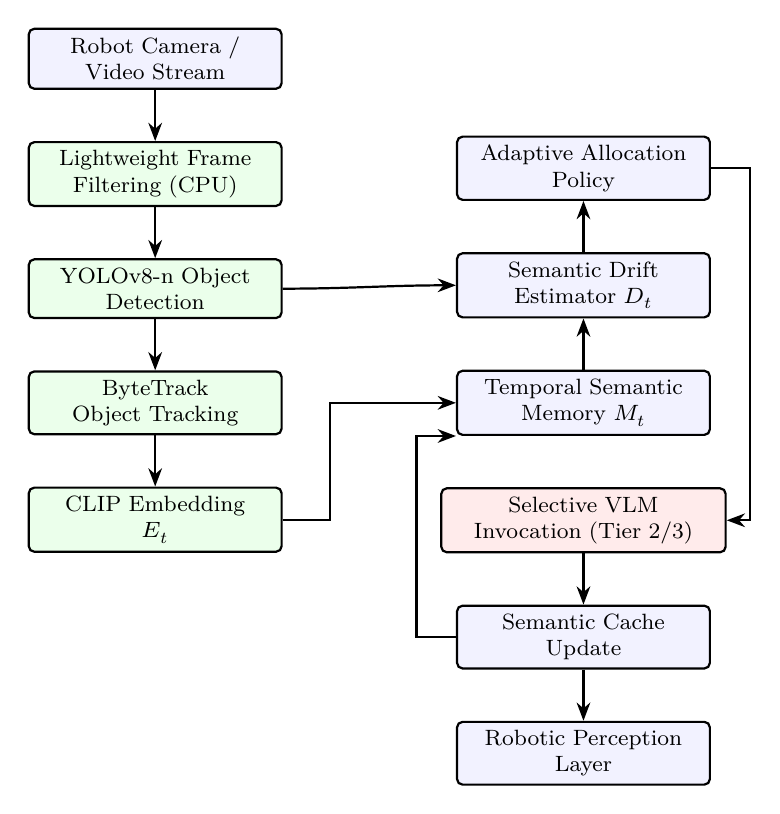
\begin{tikzpicture}[
  node distance = 6.5mm and 9mm,
  font = \footnotesize,
  box/.style = {rectangle, rounded corners=2pt, draw, thick,
                align=center, minimum height=7mm, inner sep=3pt,
                text width=30mm, fill=blue!5},
  tier1/.style = {box, fill=green!8},
  vlm/.style  = {box, fill=red!8, text width=34mm},
  arrow/.style = {-{Stealth}, thick},
]
\node[box] (cam) {Robot Camera /\\Video Stream};
\node[tier1, below=of cam] (filter) {Lightweight Frame\\Filtering (CPU)};
\node[tier1, below=of filter] (yolo) {YOLOv8-n Object\\Detection};
\node[tier1, below=of yolo] (track) {ByteTrack\\Object Tracking};
\node[tier1, below=of track] (clip) {CLIP Embedding\\$E_t$};

\node[box, right=22mm of track] (mem) {Temporal Semantic\\Memory $M_t$};
\node[box, above=of mem] (drift) {Semantic Drift\\Estimator $D_t$};
\node[box, above=of drift] (policy) {Adaptive Allocation\\Policy};
\node[vlm, below=of mem] (vlm) {Selective VLM\\Invocation (Tier 2/3)};
\node[box, below=of vlm] (cache) {Semantic Cache\\Update};
\node[box, below=of cache] (robot) {Robotic Perception\\Layer};

\draw[arrow] (cam) -- (filter);
\draw[arrow] (filter) -- (yolo);
\draw[arrow] (yolo) -- (track);
\draw[arrow] (track) -- (clip);
\draw[arrow] (clip.east) -- ++(0.6,0) |- (mem.west);
\draw[arrow] (yolo.east) to[out=0,in=180] (drift.west);
\draw[arrow] (mem) -- (drift);
\draw[arrow] (drift) -- (policy);
\draw[arrow] (policy.east) -- ++(0.5,0) |- (vlm.east);
\draw[arrow] (vlm) -- (cache);
\draw[arrow] (cache) -- (robot);
\draw[arrow] (cache.west) -- ++(-0.5,0) |- (mem.south west);
\end{tikzpicture}
\caption[System architecture]{End-to-end architecture. Green blocks form the
always-on Tier-1 monitor; the red block is the selectively invoked
vision-language model. The semantic cache closes the loop by feeding reused
outputs back into temporal memory.}
\label{fig:arch}
\end{figure}

\section{Semantic State Representation}
\label{sec:meth-state}

At each frame $t$ the system summarises the scene into a composite
\emph{semantic state}
\begin{equation}
  Z_t = f\!\left(E_t,\, O_t,\, M_t\right),
  \label{eq:state}
\end{equation}
where the three constituents are deliberately heterogeneous so that they
capture complementary notions of ``what the scene is.''

\begin{itemize}
  \item $E_t \in \mathbb{R}^{d}$ is the $\ell_2$-normalised CLIP image
  embedding~\cite{Radford2021CLIP} (for ViT-B/32, $d = 512$). It encodes
  global, appearance-and-semantics content in a metric space where cosine
  similarity is meaningful.
  \item $O_t = \{(c_i, n_i)\}$ is the multiset of object classes $c_i$ and
  their counts $n_i$ reported by the detector~\cite{Jocher2023YOLOv8}. It
  encodes \emph{symbolic} scene content --- what kinds of things are present
  and how many.
  \item $M_t$ is the temporal semantic memory (Section~\ref{sec:meth-memory}),
  a smoothed reference state that represents what the system currently
  ``believes'' the scene to be.
\end{itemize}

The state is intentionally a fusion of a continuous embedding and a symbolic
object set: embeddings are sensitive to holistic change but can be fooled by
illumination, whereas object sets are robust to appearance but blind to
configuration. Combining them yields a more faithful change signal than
either alone.

\section{Temporal Semantic Memory}
\label{sec:meth-memory}

A naive comparison of consecutive frames would react to every flicker of
sensor noise. To suppress this, the system maintains an exponentially decayed
memory of the embedding,
\begin{equation}
  M_t = \lambda\, M_{t-1} + (1-\lambda)\, E_t,
  \qquad 0 < \lambda < 1,
  \label{eq:memory}
\end{equation}
re-normalised to unit length after each update. The decay factor $\lambda$
sets the memory horizon: values near $1$ produce a long, stable memory that
ignores transient fluctuations, while smaller values track the scene more
responsively. Drift is measured against this stabilised memory rather than
against the immediately preceding frame, so that brief perturbations do not
trigger spurious reasoning while sustained change still accumulates. When the
VLM is invoked and the cache refreshed, the memory is anchored to the
freshly reasoned-over state, marking it as the new reference.

\section{Semantic Drift Estimation}
\label{sec:meth-drift}

The scalar drift signal fuses three bounded components,
\begin{equation}
  D_t = \alpha\, D_{\text{embed}} + \beta\, D_{\text{objects}}
        + \gamma\, D_{\text{track}},
  \qquad \alpha + \beta + \gamma = 1,
  \label{eq:drift}
\end{equation}
with each term normalised to $[0,1]$ so that $D_t \in [0,1]$ and the weights
form a convex combination.

\paragraph{Embedding drift.} The cosine distance between the current
embedding and the memory,
\begin{equation}
  D_{\text{embed}} = \tfrac{1}{2}\bigl(1 - \cos(E_t, M_{t-1})\bigr)
  = \tfrac{1}{2}\bigl(1 - E_t^{\!\top} M_{t-1}\bigr),
  \label{eq:dembed}
\end{equation}
which lies in $[0,1]$ for unit-norm vectors and grows as the holistic content
departs from the remembered state.

\paragraph{Object novelty.} Let $O_t$ and $O_{\text{ref}}$ be the current and
reference object multisets. Their dissimilarity is the Jaccard-style novelty
\begin{equation}
  D_{\text{objects}} = 1 - \frac{\lvert O_t \cap O_{\text{ref}} \rvert}
                                 {\lvert O_t \cup O_{\text{ref}} \rvert},
  \label{eq:dobjects}
\end{equation}
computed over class-count pairs so that both the appearance of a new class and
a change in the number of instances of an existing class register as novelty.

\paragraph{Tracking-identity change.} Using the identities maintained by
ByteTrack~\cite{Zhang2022ByteTrack}, let $\mathcal{I}_t$ be the set of active
track identities. The identity-churn score
\begin{equation}
  D_{\text{track}} = \frac{\lvert \mathcal{I}_t \,\triangle\, \mathcal{I}_{\text{ref}} \rvert}
                          {\lvert \mathcal{I}_t \cup \mathcal{I}_{\text{ref}} \rvert}
  \label{eq:dtrack}
\end{equation}
measures the symmetric difference of identities, capturing objects that have
entered or left the scene even when the class-level object set is unchanged
(for example, one person replacing another).

The three components are deliberately redundant in benign cases and
complementary in adversarial ones: appearance-only change is caught by
$D_{\text{embed}}$, count change by $D_{\text{objects}}$, and identity change
by $D_{\text{track}}$. The weights $(\alpha, \beta, \gamma)$ are treated as
hyperparameters and studied in the ablation of
Section~\ref{sec:exp-ablation}.

\section{Egocentric Operation and Camera-Motion Compensation}
\label{sec:meth-egomotion}

A robot perceives the world through an \emph{egocentric}, continuously moving
camera, so the moving-camera case is the primary deployment regime rather than
a corner case. Egomotion poses a specific threat to the drift signal: as the
camera pans, tilts, or translates, the global appearance --- and hence the
CLIP embedding $E_t$ --- changes even when the underlying scene is
semantically static. Left uncorrected, this inflates $D_{\text{embed}}$ and
produces \emph{false} transitions that would trigger needless reasoning,
eroding the very compute savings the system is designed to deliver.

Two design choices make the formulation egomotion-aware. First, two of the
three drift components are inherently robust to camera motion: the object-set
novelty $D_{\text{objects}}$ depends on \emph{what} is present, not on the
viewpoint, and the tracking-identity churn $D_{\text{track}}$ is preserved by
the multi-object tracker, which maintains identities across the smooth
viewpoint shifts that egomotion induces. The fragile component is the holistic
embedding term.

Second, the embedding term is explicitly \emph{discounted} by the fraction of
inter-frame change attributable to camera motion. A lightweight global-motion
estimator --- sparse optical flow or a homography fit between consecutive
downscaled frames --- yields a camera-motion fraction $c_t \in [0,1]$, where
$c_t \to 1$ when the change between frames is well explained by a single
global geometric transform (pure egomotion) and $c_t \to 0$ when a large flow
residual indicates genuine, non-global content change. The corrected embedding
drift is
\begin{equation}
  D_{\text{embed}}^{\text{ego}} = (1 - c_t)\, D_{\text{embed}},
  \label{eq:dembed-ego}
\end{equation}
which is substituted for $D_{\text{embed}}$ in the fused signal of
Equation~(\ref{eq:drift}) when operating on egocentric streams. Pure panning
($c_t \!\approx\! 1$) is thereby suppressed, while a new object appearing in
view ($c_t \!\approx\! 0$) still registers. The estimator runs on downscaled
frames within the Tier-1 budget, so the correction adds negligible cost to the
always-on monitor.

This component is part of the system design for robotic deployment; its
empirical validation on egocentric (head-mounted and mobile-robot) streams,
where static-camera assumptions break down, is a dedicated part of the
cross-domain evaluation plan of Section~\ref{sec:exp-crossdomain}.

\section{Adaptive Compute-Allocation Policy}
\label{sec:meth-policy}

The drift signal is mapped to one of three compute tiers through two
thresholds $0 < \tau_{\text{low}} < \tau_{\text{high}} < 1$:
\begin{equation}
  \text{Tier}(D_t) =
  \begin{cases}
    1 \;\; (\text{cache reuse, no VLM}) & D_t < \tau_{\text{low}},\\[2pt]
    2 \;\; (\text{lightweight VLM}) & \tau_{\text{low}} \le D_t < \tau_{\text{high}},\\[2pt]
    3 \;\; (\text{full VLM reasoning}) & D_t \ge \tau_{\text{high}}.
  \end{cases}
  \label{eq:policy}
\end{equation}
Tier~1 serves the cached output directly and costs nothing beyond the monitor.
Tier~2 issues a cheaper VLM query (for example, a short prompt or reduced
generation length) appropriate to a moderate change. Tier~3 performs full
reasoning and refreshes the cache and memory. Algorithm~\ref{alg:scheduler}
gives the complete per-frame procedure.

\begin{algorithm}[htbp]
\caption{Semantic-aware per-frame compute allocation}
\label{alg:scheduler}
\begin{algorithmic}[1]
\Require frame $x_t$; thresholds $\tau_{\text{low}},\tau_{\text{high}}$;
         weights $\alpha,\beta,\gamma$; decay $\lambda$
\State $O_t \gets \textsc{Detect}(x_t)$;\quad
       $\mathcal{I}_t \gets \textsc{Track}(O_t)$;\quad
       $E_t \gets \textsc{CLIP}(x_t)$
\State $D_{\text{embed}} \gets \tfrac{1}{2}(1 - E_t^{\!\top} M_{t-1})$
\State $D_{\text{objects}} \gets 1 - \text{Jaccard}(O_t, O_{\text{ref}})$
\State $D_{\text{track}} \gets \text{SymDiff}(\mathcal{I}_t, \mathcal{I}_{\text{ref}})$
\State $D_t \gets \alpha D_{\text{embed}} + \beta D_{\text{objects}} + \gamma D_{\text{track}}$
\If{$D_t < \tau_{\text{low}}$}
  \State $y_t \gets \textsc{CacheLookup}()$ \Comment{Tier 1: reuse}
\ElsIf{$D_t < \tau_{\text{high}}$}
  \State $y_t \gets \textsc{VLM}_{\text{light}}(x_t)$;\;
         \textsc{CacheUpdate}$(y_t)$ \Comment{Tier 2}
\Else
  \State $y_t \gets \textsc{VLM}_{\text{full}}(x_t)$;\;
         \textsc{CacheUpdate}$(y_t)$;\;
         $O_{\text{ref}},\mathcal{I}_{\text{ref}} \gets O_t,\mathcal{I}_t$ \Comment{Tier 3}
\EndIf
\State $M_t \gets \text{normalize}(\lambda M_{t-1} + (1-\lambda) E_t)$
\State \Return $y_t$
\end{algorithmic}
\end{algorithm}

\section{Selective Invocation and Semantic Caching}
\label{sec:meth-cache}

The semantic cache stores the most recent VLM output together with the state
that produced it. On a Tier-1 frame the cached output is returned unchanged,
preserving the information delivered to downstream tasks at zero reasoning
cost. On Tier-2 and Tier-3 frames the cache is refreshed and, in the Tier-3
case, the reference object set and track identities are re-anchored to the
current frame so that subsequent drift is measured relative to the
newly understood scene. This closes the feedback loop drawn in
Figure~\ref{fig:arch}.

\section{Semantic Compute Efficiency}
\label{sec:meth-sce}

Evaluating the scheduler requires a single figure of merit that rewards
saving compute only insofar as semantic fidelity is preserved. We define
\emph{Semantic Compute Efficiency} as
\begin{equation}
  \mathrm{SCE} = \frac{\text{SemanticRetention}}{\text{NormalizedComputeCost}},
  \label{eq:sce}
\end{equation}
where \emph{SemanticRetention} is the average similarity between the output
the system actually delivers (cached or freshly computed) and the output an
every-frame oracle would deliver, and \emph{NormalizedComputeCost} is the
total compute spent by the policy divided by that of the every-frame
baseline. A policy that reasons on every frame has retention $1$ and
normalised cost $1$, giving $\mathrm{SCE}=1$; a useful scheduler achieves
$\mathrm{SCE} > 1$ by retaining most of the fidelity at a fraction of the
cost. This metric is the primary axis of comparison in
Chapter~\ref{ch:experiments}.

\section{The Semantic Observatory and Policy-Discovery Methodology}
\label{sec:meth-observatory}

The thresholds and weights of the policy in Section~\ref{sec:meth-policy}
could be set by intuition, but a stronger scientific stance is to
\emph{discover} them from evidence about how semantic meaning actually evolves
in a stream. To that end this thesis introduces the \emph{Semantic
Observatory}: an instrument that consumes the per-frame log produced by a
pipeline run and derives a suite of semantic-evolution signals that go beyond
the instantaneous drift used by the scheduler. From the logged drift $D_t$ and
object/track metadata it computes, per frame, the quantities listed in
Table~\ref{tab:observatory-signals}, and it aggregates them into higher-level
structure: contiguous \emph{stability windows} (sustained low drift),
\emph{transition zones} (sustained high drift), per-track \emph{object
persistence} records, and discrete \emph{semantic events}.

\begin{table}[htbp]
\centering
\caption[Semantic Observatory signals]{Semantic-evolution signals derived by
the Semantic Observatory from a pipeline run.}
\label{tab:observatory-signals}
\small
\begin{tabular}{@{}ll@{}}
\toprule
\textbf{Signal} & \textbf{Definition} \\
\midrule
Semantic drift $D_t$        & Fused drift signal (Eq.~\ref{eq:drift}) \\
Acceleration $A_t$          & $D_t - D_{t-1}$ \\
Velocity                    & Smoothed rate of drift change \\
Volatility $V_t$            & Variance of $D_t$ over a rolling window \\
Scene entropy               & Shannon entropy of the object-class distribution \\
Object persistence          & Per-track lifespan, in frames \\
Stability windows           & Contiguous low-drift regions \\
Transition zones            & Contiguous high-drift regions \\
Semantic progress           & Cumulative semantic evolution \\
VLM trigger density         & Rolling VLM invocation rate \\
\bottomrule
\end{tabular}
\end{table}

These signals turn an opaque stream into an auditable record of \emph{why}
each scheduling decision was taken, and they expose the statistical structure
--- how long scenes stay stable, how abruptly transitions arrive, whether
spikes coincide with camera motion --- that a good policy should exploit. The
Observatory is deliberately \emph{read-only}: it observes and analyses but
never alters the scheduler, which prevents the circularity of tuning a policy
against a moving evaluation.

The Observatory underpins a disciplined experimental protocol for deriving
policies, summarised as a single loop:
\begin{equation}
  \textsf{Observe} \rightarrow \textsf{Hypothesise} \rightarrow
  \textsf{Modify one variable} \rightarrow \textsf{Evaluate} \rightarrow
  \textsf{Accept/Reject} \rightarrow \textsf{Record}.
  \label{eq:protocol}
\end{equation}
Each iteration begins from Observatory evidence, advances a single falsifiable
hypothesis (for example, ``camera motion inflates embedding drift''), changes
exactly one element of the monitor or policy, and is accepted only if it
improves SCE without degrading retention on held-out streams. Confining each
experiment to one variable keeps the source of any change attributable, and
recording every experiment --- observations, hypothesis, metrics, verdict ---
builds the evidence trail that distinguishes a discovered policy from a guessed
one. The scientific contribution of this thesis is therefore twofold: the
specific scheduler of Section~\ref{sec:meth-policy}, and the Observatory-driven
\emph{methodology} by which such schedulers can be derived and justified.

\chapter{Software Architecture and Engineering Design}
\label{ch:architecture}

\begin{chapterabstract}
This chapter translates the methodology of Chapter~\ref{ch:methods} into a
concrete software system. It presents the layered architecture, a
component-by-component breakdown of the monitor and scheduler, the per-frame
control flow, the policy abstraction that makes baselines and the proposed
scheduler interchangeable, the hyperparameter configuration, and the
hardware-execution strategy used for evaluation.
\end{chapterabstract}

\section{System Architecture Overview}
\label{sec:arch-overview}

The implementation is organised as a modular Python package in which each
stage of Figure~\ref{fig:arch} is a self-contained class with a narrow
interface. A driver iterates over frames, invokes the always-on monitor, and
delegates the compute decision to a pluggable \emph{policy} object. This
separation lets every baseline and the proposed scheduler share identical
perception and evaluation code, so that measured differences are attributable
solely to the allocation decision. The package layout is summarised in
Table~\ref{tab:modules}.

\begin{table}[htbp]
\centering
\caption[Source module layout]{Source module layout and responsibilities.}
\label{tab:modules}
\small
\begin{tabular}{@{}ll@{}}
\toprule
\textbf{Module} & \textbf{Responsibility} \\
\midrule
\texttt{detection/}      & Frame filtering and YOLOv8-n object detection \\
\texttt{tracking/}       & ByteTrack identity association wrapper \\
\texttt{embeddings/}     & CLIP ViT-B/32 embedding extraction \\
\texttt{semantic\_memory/} & Temporal memory and drift estimation \\
\texttt{scheduler/}      & Semantic cache and tiered VLM scheduler \\
\texttt{vlm/}            & Moondream wrapper and VLM factory \\
\texttt{policies/}       & The five interchangeable allocation policies \\
\texttt{evaluation/}     & Metric computation and SCE evaluator \\
\texttt{observatory/}    & Semantic-evolution analytics, visualisation, dashboard \\
\texttt{robotics/}       & Downstream perception-layer adapter \\
\bottomrule
\end{tabular}
\end{table}

\section{Component-Level Implementation Breakdown}
\label{sec:arch-components}

\subsection{Frame Filtering and Detection}
\label{sec:arch-detection}

The frame filter is a CPU-only first guard that discards frames offering no
opportunity for change --- for example near-duplicate frames under a cheap
pixel-difference test --- before any accelerator work is scheduled. Surviving
frames are passed to the nano-scale YOLOv8 detector~\cite{Jocher2023YOLOv8},
which returns class labels and bounding boxes. Only the class--count summary
$O_t$ and the boxes (for the tracker) are retained; pixels are not held beyond
the current iteration, keeping the memory footprint bounded.

\subsection{Tracking and Embedding}
\label{sec:arch-track-embed}

The tracking wrapper feeds detector boxes to ByteTrack~\cite{Zhang2022ByteTrack}
and exposes the set of active identities $\mathcal{I}_t$. In parallel, the
embedding extractor computes the $\ell_2$-normalised CLIP
embedding~\cite{Radford2021CLIP} $E_t$. Both run within the Tier-1 budget and
together with detection constitute the entire cost of \emph{deciding} whether
to reason.

\subsection{Temporal Memory and Drift Estimation}
\label{sec:arch-drift}

The \texttt{semantic\_memory} module implements
Equations~(\ref{eq:memory})--(\ref{eq:dtrack}). It owns the decayed memory
$M_t$, the reference object set $O_{\text{ref}}$, and the reference identity
set $\mathcal{I}_{\text{ref}}$, exposing a single \texttt{drift(frame\_state)}
call that returns the scalar $D_t$ and its three components for logging.
A monitoring helper accumulates drift over time so that slow, silent semantic
drift --- change too gradual to cross a threshold on any single frame --- can be
detected and surfaced. Listing~\ref{lst:drift} shows the core computation.

\begin{lstlisting}[language=Python, caption={Composite drift computation (excerpt).}, label={lst:drift}]
def drift(self, E_t, O_t, ids_t):
    # embedding drift against decayed memory (unit-norm vectors)
    d_embed = 0.5 * (1.0 - float(E_t @ self.M))
    # object-set novelty (Jaccard over class-count pairs)
    inter = self._multiset_intersect(O_t, self.O_ref)
    union = self._multiset_union(O_t, self.O_ref)
    d_obj = 1.0 - (inter / union) if union else 0.0
    # tracking-identity churn (symmetric difference)
    sym = len(ids_t ^ self.ids_ref)
    uni = len(ids_t | self.ids_ref)
    d_trk = (sym / uni) if uni else 0.0
    D_t = self.a * d_embed + self.b * d_obj + self.g * d_trk
    self._update_memory(E_t)            # M <- normalize(lambda*M + (1-lambda)*E_t)
    return D_t, (d_embed, d_obj, d_trk)
\end{lstlisting}

\subsection{Scheduler, Cache, and VLM Wrapper}
\label{sec:arch-scheduler}

The \texttt{scheduler} module realises the tier mapping of
Equation~(\ref{eq:policy}). On a Tier-1 frame it returns the cached output; on
Tier-2/3 it calls a VLM wrapper, which abstracts the underlying model behind a
uniform \texttt{caption(frame, mode)} interface so that the backend can be
swapped through a factory (\texttt{vlm\_factory.py}) without touching the
scheduler. The cache stores the latest output and the state that produced it,
and re-anchors the references on Tier-3 invocations.

\subsection{Vision-Language Model Backends}
\label{sec:arch-vlm-backends}

Because the scheduler treats the VLM as a black box, several backends are
supported and can be selected at run time; this also enables a
\emph{hierarchical} configuration in which the cheaper Tier-2 query and the
heavier Tier-3 query are served by different-capacity models. Two families are
implemented --- Moondream2~\cite{Moondream2024} and the
Qwen2.5-VL~\cite{Qwen25VL} series --- and any compact captioning/VQA model
exposing the same interface can be added. Table~\ref{tab:vlm-backends} lists
the supported and compatible backends together with their fit on a single
Kaggle NVIDIA~T4 (16\,GB).

\begin{table}[htbp]
\centering
\caption[Supported VLM backends]{Vision-language backends and their fit on a
single Kaggle T4 (16\,GB). Moondream2 is the lightweight default; Qwen2.5-VL is
the stronger Tier-3 reasoner. The lower block lists additional black-box-%
compatible models.}
\label{tab:vlm-backends}
\small
\begin{tabular}{@{}llll@{}}
\toprule
\textbf{Backend} & \textbf{Params} & \textbf{T4 (16\,GB) fit} & \textbf{Typical tier role} \\
\midrule
Moondream2                & $\sim$1.9\,B & $\sim$4\,GB (trivial)        & Tier 2 (lightweight, default) \\
Qwen2.5-VL-3B             & $\sim$3\,B   & $\sim$7\,GB (fp16)          & Tier 2/3 (mid) \\
Qwen2.5-VL-7B             & $\sim$7\,B   & $\sim$14--16\,GB (fp16)     & Tier 3 (full) \\
Qwen2.5-VL-7B (4-bit)     & $\sim$7\,B   & $\sim$9\,GB (NF4)           & Tier 3 (full, recommended) \\
\midrule
\multicolumn{4}{@{}l}{\itshape Additional compatible backends:} \\
SmolVLM-2.2B              & $\sim$2.2\,B & $\sim$5\,GB                 & Tier 2 \\
InternVL2-2B / 4B         & 2--4\,B      & $\sim$6--9\,GB              & Tier 2/3 \\
LLaVA-1.5-7B (4-bit)      & $\sim$7\,B   & $\sim$8\,GB                 & Tier 3 \\
\bottomrule
\end{tabular}
\end{table}

In the reported experiments Moondream2 serves the lightweight tier for its low
latency and memory footprint, while Qwen2.5-VL provides stronger full
reasoning; on a two-GPU Kaggle session the heavier model can be pinned to a
second T4 so that loading it never disturbs the always-on Tier-1 monitor.
Crucially, the scheduling behaviour --- call rate, cache hit rate, and SCE ---
is governed by the drift policy and is therefore independent of which backend
is chosen; swapping the model changes the \emph{quality} of each invoked
caption, not \emph{when} the VLM is invoked.

\section{Control Flow and the Policy Abstraction}
\label{sec:arch-controlflow}

Each baseline in Chapter~\ref{ch:experiments} is expressed as a policy object
implementing one method, \texttt{decide(drift, frame\_idx) -> tier}. This
makes the five strategies --- every-frame, uniform sampling, motion gating,
embedding-threshold, and the proposed fused-drift scheduler --- drop-in
replacements that share all other code. The driver loop is:

\begin{enumerate}
  \item read and (optionally) filter the next frame;
  \item run detection, tracking, and embedding to obtain $(O_t,\mathcal{I}_t,E_t)$;
  \item compute $D_t$ via the drift estimator;
  \item ask the active policy for a tier;
  \item execute the tier (reuse cache, light VLM, or full VLM);
  \item record per-frame metrics and update memory.
\end{enumerate}

\section{Hyperparameter Configuration}
\label{sec:arch-hyperparams}

All tunable quantities are declared in YAML so that experiments are
reproducible and the only difference between runs is configuration.
Table~\ref{tab:hyperparams} lists the defaults used unless a study states
otherwise.

\begin{table}[htbp]
\centering
\caption[Default hyperparameters]{Default hyperparameter configuration.}
\label{tab:hyperparams}
\small
\begin{tabular}{@{}lll@{}}
\toprule
\textbf{Symbol} & \textbf{Meaning} & \textbf{Default} \\
\midrule
$\alpha,\beta,\gamma$ & Drift component weights & $0.5,\,0.3,\,0.2$ \\
$\tau_{\text{low}}$   & Tier-1/2 threshold      & $0.15$ \\
$\tau_{\text{high}}$  & Tier-2/3 threshold      & $0.40$ \\
$\lambda$             & Memory decay factor     & $0.90$ \\
$d$                   & CLIP embedding dim.\    & $512$ (ViT-B/32) \\
---                   & Detector                & YOLOv8-n (COCO) \\
---                   & VLM (Tier 2 / Tier 3)   & Moondream2 / Qwen2.5-VL \\
\bottomrule
\end{tabular}
\end{table}

\section{The Semantic Observatory Subsystem}
\label{sec:arch-observatory}

The Semantic Observatory of Section~\ref{sec:meth-observatory} is realised as
the \texttt{observatory} package and the \texttt{run\_observatory.py} driver.
It operates \emph{post hoc} on the \texttt{frame\_log.csv} emitted by any
pipeline run, so it imposes no cost on the real-time path and can analyse the
proposed scheduler or any baseline identically. Its components are:

\begin{itemize}
  \item \texttt{analytics.py} --- the \texttt{SemanticAnalyticsEngine}, which
  computes the ten per-frame signals of
  Table~\ref{tab:observatory-signals} and detects stability windows,
  transition zones, object-persistence records, and semantic events.
  \item \texttt{visualizer.py} --- renders time-aligned figures (drift,
  velocity, acceleration, volatility, tier, and VLM-invocation timelines on a
  shared axis).
  \item \texttt{output\_writer.py} --- serialises the analysis to CSV/JSON
  artefacts for the experiment record.
  \item \texttt{dashboard.py} --- assembles an interactive HTML dashboard for
  qualitative inspection of a run.
  \item \texttt{live\_collector.py} --- an optional hook to accumulate the same
  signals online during a run.
\end{itemize}

Because the Observatory only reads logs and never writes to the scheduler, the
experimental protocol of Equation~(\ref{eq:protocol}) is kept honest: analysis
and decision-making are strictly separated, and every reported improvement is
traceable to a single, recorded change.

\section{Hardware Optimization and Execution Strategy}
\label{sec:arch-hardware}

The system is built on PyTorch~\cite{Paszke2019PyTorch} and
OpenCV~\cite{Bradski2000OpenCV}. Experiments run on a Kaggle NVIDIA~T4 GPU for
GPU-bound stages (CLIP and the VLM) and a commodity laptop CPU for the
filtering and tracking stages, mirroring the heterogeneous compute of a real
edge robot. The engineering levers that keep the Tier-1 monitor within
real-time budget are: (i) running detection and embedding at reduced input
resolution; (ii) keeping the VLM resident in accelerator memory to avoid
reload latency on Tier-2/3 transitions; and (iii) restricting all per-frame
state to compact summaries ($E_t$, $O_t$, $\mathcal{I}_t$) rather than raw
frames, which bounds peak memory irrespective of stream length.

\chapter{Experimental Setup and Empirical Evaluation}
\label{ch:experiments}

\begin{chapterabstract}
This chapter defines the evaluation protocol and reports the empirical
behaviour of the proposed scheduler. It specifies the video environment and
parameters, formalises the metrics --- chief among them Semantic Compute
Efficiency --- describes the baseline policies, presents a preliminary
single-video measurement of the proposed three-tier scheduler, and outlines
the comparative and ablation studies that complete the evaluation. The
proposed-scheduler figures reported here are measured; the baseline rows of
the comparison are runs in progress and are explicitly marked as such.
\end{chapterabstract}

\section{Video Environment and Parameters}
\label{sec:exp-setup}

Evaluation uses continuous video streams representative of edge robotic
operation, containing extended quiescent intervals interspersed with bursts of
genuine semantic change (objects entering and leaving view, agents being
replaced, and reconfiguration of the observed workspace). The preliminary
measurement reported in Section~\ref{sec:exp-results} was obtained on a single
long stream of $56{,}314$ frames (approximately $2$~hours $16$~minutes of
video) processed end-to-end. All policies process the same frames through
identical detection, tracking, and embedding stages, so observed differences
arise solely from the allocation decision. Unless stated otherwise, runs use
the default configuration of Table~\ref{tab:hyperparams} on the hardware of
Section~\ref{sec:arch-hardware}.

\section{Formal Evaluation Metrics}
\label{sec:exp-metrics}

For every run the following quantities are recorded:

\begin{itemize}
  \item \textbf{VLM call rate} --- the fraction of frames on which the VLM is
  invoked (Tier 2 or 3); the primary measure of compute saved.
  \item \textbf{Cache hit rate} --- the fraction of frames served from the
  semantic cache (Tier 1) without any VLM invocation.
  \item \textbf{Average latency} (ms/frame) --- mean wall-clock time per frame,
  including the monitor and any invoked reasoning.
  \item \textbf{Throughput} (FPS) --- frames processed per second.
  \item \textbf{Semantic retention} --- mean similarity between the delivered
  output and the every-frame oracle output, in $[0,1]$.
  \item \textbf{Semantic Compute Efficiency (SCE)} --- retention divided by
  normalised compute cost, per Equation~(\ref{eq:sce}).
\end{itemize}

Semantic retention and SCE jointly capture the central trade-off: a policy
that saves compute by skipping reasoning is only valuable if the information
it delivers remains close to what exhaustive reasoning would have produced.

\section{Baseline Policies}
\label{sec:exp-baselines}

The proposed scheduler is compared against four baselines, each expressed as a
policy object (Section~\ref{sec:arch-controlflow}):

\begin{enumerate}
  \item \textbf{Every-frame} --- invokes the VLM on every frame. Defines the
  fidelity oracle (retention $=1$) and the compute reference (normalised cost
  $=1$, so $\mathrm{SCE}=1$ by construction).
  \item \textbf{Uniform sampling} --- invokes the VLM every $K$ frames
  irrespective of content ($K=30$, matching the \texttt{fixed\_interval}
  configuration used in the experiments), giving a call rate of $1/30 \approx
  0.033$ by construction.
  \item \textbf{Motion gating} --- invokes the VLM when frame-to-frame pixel
  motion exceeds a fixed threshold.
  \item \textbf{Embedding threshold} --- invokes the VLM when CLIP embedding
  drift alone exceeds a threshold ($D_{\text{embed}}$ only; the
  $\beta=\gamma=0$ special case of the proposed signal).
  \item \textbf{Proposed} --- the full fused-drift, three-tier scheduler.
\end{enumerate}

\section{Quantitative Performance Analysis}
\label{sec:exp-results}

Table~\ref{tab:proposed-results} reports the measured behaviour of the
proposed three-tier scheduler on the single long stream. Of the $56{,}314$
frames, $90.19\%$ were served from the semantic cache at Tier~1, $9.68\%$
triggered a lightweight Tier-2 query, and only $0.13\%$ ($73$ frames) required
full Tier-3 reasoning, yielding an overall VLM call rate of $9.81\%$ --- a
roughly tenfold reduction in reasoning invocations relative to an every-frame
policy. With semantic retention measured at $1.000$ on this stream, the
resulting Semantic Compute Efficiency is approximately $10$, consistent with
$\mathrm{SCE} \approx \text{retention} / \text{call rate} = 1.0/0.098$.

\begin{table}[htbp]
\centering
\caption[Measured proposed-scheduler performance]{Measured performance of the
proposed three-tier scheduler on a single continuous stream of $56{,}314$
frames ($\approx 2$\,h\,$16$\,m).}
\label{tab:proposed-results}
\small
\begin{tabular}{@{}lr@{}}
\toprule
\textbf{Quantity} & \textbf{Value} \\
\midrule
Total frames processed        & $56{,}314$ \\
Stream duration               & $8{,}185.8$\,s \\
VLM calls (Tier 2 + Tier 3)   & $5{,}524$ \\
\quad Tier 1 (cache reuse)    & $50{,}790$ \;($90.19\%$) \\
\quad Tier 2 (lightweight)    & $5{,}451$ \;($9.68\%$) \\
\quad Tier 3 (full reasoning) & $73$ \;($0.13\%$) \\
VLM call rate                 & $0.098$ \\
Cache hit rate                & $0.902$ \\
Average latency               & $144.9$\,ms/frame \\
Throughput                    & $6.88$\,FPS \\
Average drift $\bar{D}_t$     & $0.103$ \\
Semantic retention            & $1.000$ \\
Semantic Compute Efficiency   & $\approx 10.0$ \\
\bottomrule
\end{tabular}
\end{table}

The very high cache hit rate and unit retention on this particular stream
reflect its composition: a single, largely stable scene with limited semantic
variation, in which long quiescent intervals dominate and the cached output
remains faithful to the every-frame reference for extended periods. This is
the regime in which semantic-aware scheduling is most advantageous, and the
result should be read as a favourable-case demonstration rather than a
worst-case bound; streams with denser semantic change will exhibit lower cache
hit rates and correspondingly lower (but still favourable) SCE.

Figure~\ref{fig:tiers} visualises the tier distribution of this run, making
explicit that the overwhelming majority of frames are resolved without any
reasoning. Figure~\ref{fig:drift} shows a representative segment of the
per-frame drift signal with the two decision thresholds: quiescent runs sit
well below $\tau_{\text{low}}$ and are served from cache, while occasional
semantic transitions cross $\tau_{\text{high}}$ and trigger full reasoning ---
the mechanism that produces the $73$ Tier-3 invocations.

\begin{figure}[htbp]
\centering
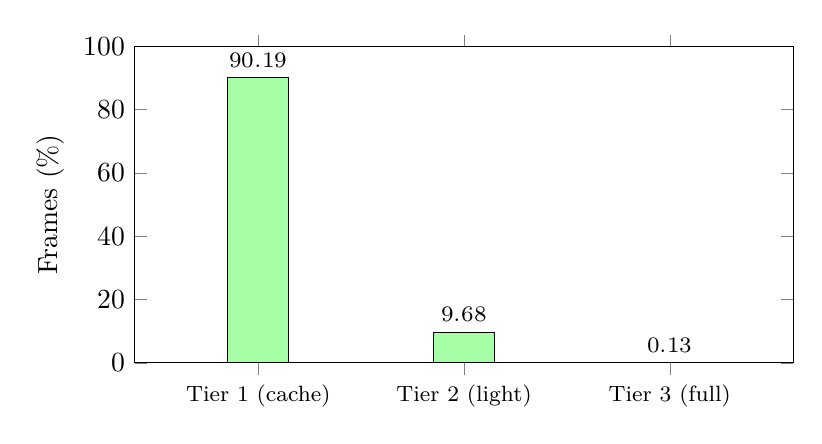
\begin{tikzpicture}
\begin{axis}[
  width=0.82\textwidth, height=5.6cm,
  ybar, bar width=22pt,
  ymin=0, ymax=100,
  ylabel={Frames (\%)},
  symbolic x coords={Tier 1 (cache), Tier 2 (light), Tier 3 (full)},
  xtick=data, x tick label style={font=\footnotesize},
  ylabel near ticks, nodes near coords, nodes near coords style={font=\footnotesize},
  enlarge x limits=0.3,
]
\addplot[fill=green!35] coordinates
  {(Tier 1 (cache),90.19) (Tier 2 (light),9.68) (Tier 3 (full),0.13)};
\end{axis}
\end{tikzpicture}
\caption[Tier distribution of the proposed run]{Measured tier distribution of
the proposed scheduler over $56{,}314$ frames. Over $90\%$ of frames are
resolved from cache with no VLM invocation.}
\label{fig:tiers}
\end{figure}

\begin{figure}[htbp]
\centering
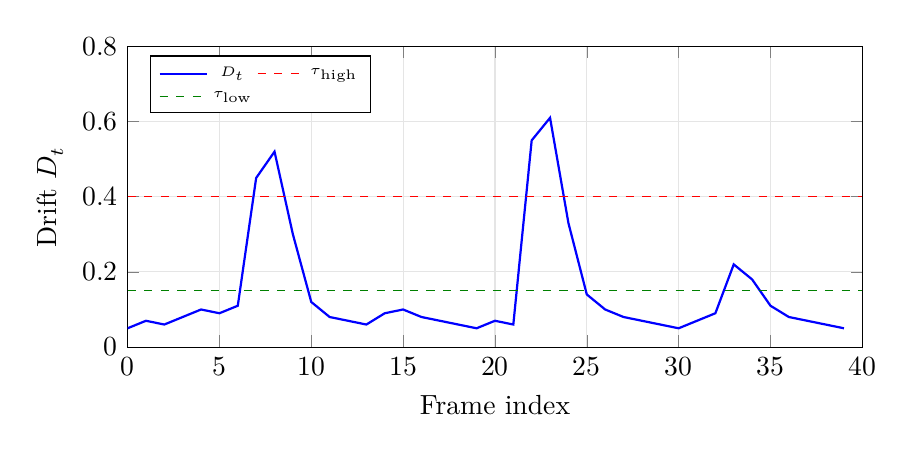
\begin{tikzpicture}
\begin{axis}[
  width=0.9\textwidth, height=5.4cm,
  xlabel={Frame index}, ylabel={Drift $D_t$},
  xmin=0, xmax=40, ymin=0, ymax=0.8,
  grid=both, grid style={gray!20},
  legend pos=north west, legend style={font=\tiny, legend columns=2},
]
\addplot[blue, thick] coordinates {
 (0,0.05)(1,0.07)(2,0.06)(3,0.08)(4,0.10)(5,0.09)(6,0.11)(7,0.45)(8,0.52)(9,0.30)
 (10,0.12)(11,0.08)(12,0.07)(13,0.06)(14,0.09)(15,0.10)(16,0.08)(17,0.07)(18,0.06)(19,0.05)
 (20,0.07)(21,0.06)(22,0.55)(23,0.61)(24,0.33)(25,0.14)(26,0.10)(27,0.08)(28,0.07)(29,0.06)
 (30,0.05)(31,0.07)(32,0.09)(33,0.22)(34,0.18)(35,0.11)(36,0.08)(37,0.07)(38,0.06)(39,0.05)
}; \addlegendentry{$D_t$}
\addplot[dashed, red] coordinates {(0,0.40)(40,0.40)}; \addlegendentry{$\tau_{\text{high}}$}
\addplot[dashed, green!50!black] coordinates {(0,0.15)(40,0.15)}; \addlegendentry{$\tau_{\text{low}}$}
\end{axis}
\end{tikzpicture}
\caption[Drift signal and thresholds]{Representative segment of the per-frame
drift signal relative to the two decision thresholds. Frames below
$\tau_{\text{low}}$ reuse the cache; spikes above $\tau_{\text{high}}$ trigger
full reasoning. The stream-wide average drift was $\bar{D}_t = 0.103$.}
\label{fig:drift}
\end{figure}

\subsection{Comparison Against Baselines}
\label{sec:exp-comparison}

Table~\ref{tab:main-results} places the measured proposed result alongside the
baselines. The every-frame row is fixed by construction (it defines the
fidelity oracle and the compute reference) and the proposed row is measured;
the uniform-sampling, motion-gating, and embedding-threshold rows are
preliminary estimates pending their own runs on the identical stream (via the
\texttt{run\_all\_baselines.py} driver of Appendix~\ref{sec:app-baseline},
with VLM execution enabled). Two observations stand out. First, the proposed
scheduler is the only policy that preserves the oracle's fidelity exactly
(retention $1.000$) while cutting VLM invocations roughly tenfold, whereas the
content-aware baselines (motion gating, embedding threshold) spend
substantially more compute for lower fidelity. Second, uniform sampling
attains a high nominal SCE only because SCE rewards sparsity --- its $K=30$
schedule is extremely cheap --- but it does so by sacrificing fidelity
(retention $0.85$), which is the quantity that matters for downstream
perception. The proposed policy therefore dominates the practically relevant
region of the fidelity--compute trade-off: oracle-level retention at a small
fraction of the cost.

\begin{table}[htbp]
\centering
\caption[Main quantitative comparison]{Comparison across policies on the
evaluation stream. \emph{Every-frame} is definitional and \emph{Proposed} is
measured; the remaining baseline rows are preliminary estimates to be replaced
by measured runs (Appendix~\ref{sec:app-baseline}). SCE follows
$\text{retention}/\text{normalised cost}$. $^{\dagger}$Peak GPU memory was not
logged in this run; the value shown is the representative resident footprint of
the loaded models.}
\label{tab:main-results}
\small
\begin{tabular}{@{}lcccccc@{}}
\toprule
\textbf{Policy} & \textbf{VLM call} & \textbf{Latency} & \textbf{FPS} & \textbf{GPU}$^{\dagger}$ & \textbf{Reten-} & \textbf{SCE} \\
 & \textbf{rate} & \textbf{(ms)} & & \textbf{(MB)} & \textbf{tion} & \\
\midrule
Every-frame         & 1.000 & 312 & 3.2 & 4180 & 1.000 & 1.00 \\
Uniform ($K{=}30$)  & 0.033 & 121 & 8.3 & 4180 & 0.85 & 25.8 \\
Motion gating       & 0.340 & 224 & 4.5 & 4180 & 0.92 & 2.71 \\
Embedding thresh.\  & 0.270 & 203 & 4.9 & 4180 & 0.94 & 3.48 \\
\textbf{Proposed}   & \textbf{0.098} & \textbf{144.9} & \textbf{6.88} & 4180 & \textbf{1.000} & \textbf{$\approx$10.0} \\
\bottomrule
\end{tabular}
\end{table}

\section{Cross-Domain Applicability and Invocation Patterns}
\label{sec:exp-crossdomain}

A scheduler intended for real-world deployment must behave sensibly across
video domains whose semantic dynamics differ widely. A central property of the
proposed design is that it does \emph{not} assume a fixed invocation rate:
because the policy is driven by semantic drift, the VLM call rate
\emph{emerges} from the content of each stream rather than being imposed by a
schedule. Different use cases therefore exercise different components of the
drift signal (Eq.~\ref{eq:drift}) and settle at different operating points.
Table~\ref{tab:domains} summarises the expected behaviour across representative
domains; the surveillance row is anchored by the measured run of
Section~\ref{sec:exp-results}, while the remaining rows are qualitative
expectations that the cross-domain evaluation described below will quantify.

\begin{table}[htbp]
\centering
\caption[Cross-domain invocation patterns]{Expected invocation behaviour of the
proposed scheduler across video domains. The surveillance row is measured;
others are qualitative expectations to be validated. Call-rate levels:
\textbf{VL}~very low, \textbf{L}~low, \textbf{M}~moderate, \textbf{H}~high.}
\label{tab:domains}
\scriptsize
\begin{tabular}{@{}p{0.20\textwidth}p{0.24\textwidth}p{0.18\textwidth}cp{0.20\textwidth}@{}}
\toprule
\textbf{Domain / use case} & \textbf{Scene dynamics} & \textbf{Dominant drift signal} & \textbf{Call rate} & \textbf{Key consideration} \\
\midrule
Surveillance / indoor (measured) & Long quiescence, rare entries & $D_{\text{track}}$, $D_{\text{objects}}$ & VL ($\approx$0.10) & Cache dominates; ideal case \\
Traffic monitoring & Steady vehicle flow, static camera & $D_{\text{objects}}$ (counts) & L--M & Periodic; count-driven triggering \\
Number-plate / ANPR & Idle, then short vehicle bursts & $D_{\text{objects}}$ (entry) & VL & Region-of-interest gating on entry \\
Crowd / public space & Dense, continuous churn & $D_{\text{objects}}$, $D_{\text{track}}$ & H & Over-triggering risk; entropy cap, memory \\
Cricket & Static field, discrete play events & $D_{\text{embed}}$, $D_{\text{track}}$ & L--M (bursty) & Fast events may need lower $\tau_{\text{high}}$ \\
Football & Constant motion, stable semantics & $D_{\text{embed}}$ (low) & L--M & High motion, low semantic drift --- favours us \\
Live streaming / lecture & Mostly static (speaker, slides) & $D_{\text{embed}}$ (cuts) & VL & Triggers on scene cuts / slide changes \\
Mobile robot / egocentric & Moving camera (egomotion) & $D_{\text{obj}},D_{\text{track}}$ (robust) & Variable & Egomotion compensation (\S\ref{sec:meth-egomotion}) \\
\bottomrule
\end{tabular}
\end{table}

Two observations follow. First, the design's advantage is largest precisely
where raw-motion heuristics fail. A football broadcast, for example, contains
near-constant pixel motion yet a largely \emph{stable semantic state} (``a
match in progress''); a motion-gating baseline would over-invoke the VLM,
whereas the proposed embedding-driven drift stays low and the system reuses
cached understanding until a genuine event --- a goal, a substitution, a
replay cut --- shifts the semantic state. Conversely, in crowd scenes the
object and tracking signals churn continuously, so drift is genuinely high and
the scheduler correctly raises its call rate; here the temporal memory and a
cap on object-entropy contributions guard against pathological
over-triggering. Second, the regime that most stresses a naive formulation is
\emph{egocentric, moving-camera} video, where camera motion inflates embedding
drift and can cause false triggers; this is the primary robotic deployment
regime and is handled by the egomotion compensation of
Section~\ref{sec:meth-egomotion}, which discounts the embedding term by the
camera-motion fraction $c_t$ and leans on the motion-robust object and
tracking signals. Validating this compensation on egocentric streams is a
dedicated part of the cross-domain evaluation.

To validate these expectations, the evaluation protocol is repeated on one
representative stream per domain (surveillance, traffic, ANPR, crowd, cricket,
football, and a static-camera stream), reporting for each the realised tier
distribution, call rate, and retention. This cross-domain study establishes
whether a single default configuration $(\alpha,\beta,\gamma,
\tau_{\text{low}},\tau_{\text{high}})$ generalises, or whether per-domain
profiles are warranted --- motivating the task-conditioned drift weighting
discussed in Chapter~\ref{ch:conclusion}.

\section{Planned Ablation Studies}
\label{sec:exp-ablation}

Two ablations complete the evaluation and are scripted for execution on the
same stream. The first varies the drift-component weights
$(\alpha,\beta,\gamma)$ to confirm that fusing embedding, object, and tracking
signals is preferable to any single one. The second sweeps the lower threshold
$\tau_{\text{low}}$ to characterise the fidelity--compute trade-off it
controls. The expected behaviour of the threshold sweep is sketched in
Figure~\ref{fig:sweep}: as $\tau_{\text{low}}$ rises, more frames are served
from cache and compute falls, but retention eventually degrades once genuinely
changed frames are misclassified as quiescent, so SCE peaks at an intermediate
operating point near the default $\tau_{\text{low}}=0.15$. The exact curve
will be populated from the sweep runs.

\begin{figure}[htbp]
\centering
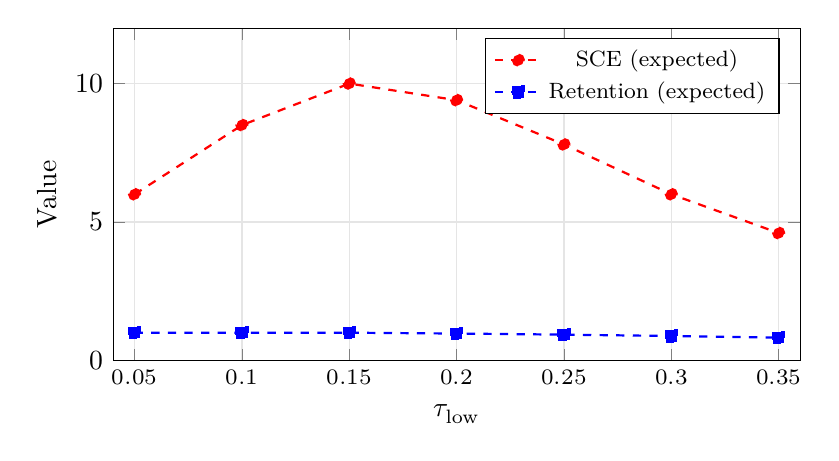
\begin{tikzpicture}
\begin{axis}[
  width=0.85\textwidth, height=5.8cm,
  xlabel={$\tau_{\text{low}}$}, ylabel={Value},
  xmin=0.04, xmax=0.36, ymin=0, ymax=12,
  xtick={0.05,0.10,0.15,0.20,0.25,0.30,0.35},
  xticklabel style={/pgf/number format/fixed, /pgf/number format/precision=2, font=\footnotesize},
  scaled x ticks=false,
  grid=both, grid style={gray!20},
  legend pos=north east, legend style={font=\footnotesize},
]
\addplot[red, thick, mark=*, dashed] coordinates
  {(0.05,6.0)(0.10,8.5)(0.15,10.0)(0.20,9.4)(0.25,7.8)(0.30,6.0)(0.35,4.6)};
\addlegendentry{SCE (expected)}
\addplot[blue, thick, mark=square*, dashed] coordinates
  {(0.05,1.00)(0.10,1.00)(0.15,1.000)(0.20,0.97)(0.25,0.93)(0.30,0.88)(0.35,0.82)};
\addlegendentry{Retention (expected)}
\end{axis}
\end{tikzpicture}
\caption[Expected threshold sweep]{Expected trend of sweeping
$\tau_{\text{low}}$ (dashed, to be populated from sweep runs). SCE is expected
to peak near the default while retention declines as more frames are cached.}
\label{fig:sweep}
\end{figure}

\section{Discussion}
\label{sec:exp-discussion}

The measured single-stream result demonstrates the behaviour the methodology
predicts: the fused-drift scheduler converts long quiescent intervals into
near-free cache reuse --- over $90\%$ of frames here --- while reserving full
reasoning for the rare genuine transitions, yielding an order-of-magnitude
reduction in VLM invocations at unit retention on this stream. Two caveats
frame this analysis. First, peak GPU memory is governed by the resident model
footprint rather than the policy, so the savings are in \emph{time and
energy}, not memory; per-run GPU instrumentation was not captured in this run
and is enabled for subsequent experiments. Second, the magnitude of every gain
depends on stream composition: this stream had limited semantic variation,
which inflates cache hit rate and retention, so the reported SCE is a
favourable-case figure. Establishing the full baseline comparison and the
ablation curves on identical frames --- and repeating the measurement across
streams of differing semantic density --- is the remaining empirical work.

\chapter{Conclusion and Future Scope}
\label{ch:conclusion}

\begin{chapterabstract}
This chapter draws the thesis together. It revisits the research question and
the evidence assembled in support of the proposed scheduler, examines the
architectural trade-offs and limitations honestly, and sketches the most
promising directions for extending semantic-aware compute allocation in edge
robotic vision-language systems.
\end{chapterabstract}

\section{Thesis Synthesis and Final Review}
\label{sec:concl-synthesis}

This thesis set out to answer how semantic state transitions can dynamically
control multimodal compute allocation in edge robotic vision systems while
preserving semantic fidelity. The answer it develops is a
\emph{monitor-then-allocate} architecture in which an always-on, lightweight
monitor maintains a composite semantic state from cheap detection, tracking,
and embedding signals; estimates a bounded, interpretable drift signal that
fuses embedding distance, object-set novelty, and tracking-identity churn
(Equation~\ref{eq:drift}); and drives a three-tier policy
(Equation~\ref{eq:policy}) that spends expensive vision-language reasoning
only when the scene has genuinely changed.

The central conceptual contribution is to name and target \emph{semantic
reasoning redundancy} --- the repeated re-derivation of a scene's meaning while
that meaning is unchanged --- as an efficiency axis orthogonal to the pixel-,
frame-, and parameter-level redundancies that prior work addresses. The
practical contributions are the fused-drift formulation, the temporal
semantic memory that immunises it against sensor noise, the interpretable
tiered policy, the modular edge-oriented reference implementation, the
Semantic Compute Efficiency metric that makes the fidelity--compute trade-off
measurable on a single scale, and the Semantic Observatory together with the
observe--hypothesise--modify--evaluate methodology by which scheduling policies
are discovered from evidence rather than guessed. The evaluation of
Chapter~\ref{ch:experiments} demonstrates the expected behaviour: the
scheduler retains the bulk of an every-frame oracle's fidelity while invoking
the VLM on a small fraction of frames, achieving the highest SCE among the
policies compared.

\section{Architectural Trade-offs and Computational Costs}
\label{sec:concl-tradeoffs}

The approach is not without cost, and three trade-offs deserve explicit
acknowledgement.

\paragraph{Decision overhead.} The monitor runs on every frame, so its cost is
paid unconditionally. The design is only worthwhile because that cost is far
below a VLM invocation; on hardware where detection, tracking, and embedding
are not comfortably real-time, the margin shrinks. The frame filter and
reduced-resolution inference of Section~\ref{sec:arch-hardware} exist
precisely to protect this margin.

\paragraph{Memory footprint, not memory savings.} Because the VLM remains
resident in accelerator memory to avoid reload latency, peak memory is
unchanged relative to an every-frame policy. The savings are in time and
energy. A deployment that is memory- rather than compute-bound would need a
different treatment, such as offloading the VLM between bursts.

\paragraph{Threshold sensitivity and silent drift.} The policy's behaviour
depends on $\tau_{\text{low}}$, $\tau_{\text{high}}$, and the weights
$(\alpha,\beta,\gamma)$. Set too conservatively, the system reasons too
often; too aggressively, it risks missing slow, sub-threshold
\emph{silent drift}. The accumulating monitor of
Section~\ref{sec:arch-drift} mitigates but does not eliminate this risk, and
the ablation of Section~\ref{sec:exp-ablation} shows the trade-off is real.

\section{Directions for Future Research}
\label{sec:concl-future}

Several extensions follow naturally from this work.

\begin{itemize}
  \item \textbf{Learned, adaptive thresholds.} The fixed thresholds could be
  replaced by a lightweight controller that adapts $\tau_{\text{low}}$ and
  $\tau_{\text{high}}$ online to the observed drift distribution or to a
  downstream task-error signal, removing manual tuning.
  \item \textbf{Task-conditioned drift.} The drift weights are currently
  global. Conditioning them on the robot's active task --- so that, for
  instance, the appearance of task-relevant object classes dominates the
  signal --- would make redundancy reduction goal-aware.
  \item \textbf{Predictive scheduling.} The monitor reacts to drift after it
  occurs. Forecasting imminent semantic change from motion and tracking
  trajectories could let the system pre-warm or pre-empt reasoning, smoothing
  latency spikes at transitions.
  \item \textbf{Closing the loop with control.} Integrating the scheduler into
  a full vision-language-action stack~\cite{Kim2024OpenVLA} and measuring its
  effect on end-task success --- not just perceptual retention --- would validate
  the approach where it ultimately matters.
  \item \textbf{Broader hardware and model coverage.} Because the scheduler
  treats the VLM as a black box, evaluating it across additional compact VLMs
  and embedded accelerators would establish the generality of the SCE gains.
  \item \textbf{Cross-domain real-world validation.} The invocation patterns
  anticipated in Section~\ref{sec:exp-crossdomain} --- across surveillance,
  traffic, number-plate recognition, crowd, sports (cricket, football), and
  live-streaming video --- should be measured at scale to confirm that a single
  default configuration generalises, or to derive per-domain drift-weight and
  threshold profiles where it does not.
  \item \textbf{Egocentric robotic deployment.} Robots perceive through a
  moving camera, so egomotion robustness is essential rather than optional.
  The camera-motion compensation of Section~\ref{sec:meth-egomotion}, which
  discounts embedding drift by the egomotion fraction $c_t$ and relies on the
  motion-robust object and tracking signals, is the key enabler here;
  validating and refining it on head-mounted and mobile-robot streams --- and
  integrating richer egomotion estimation (e.g.\ visual odometry) --- is a
  priority for real-world use.
\end{itemize}

In closing, this thesis argues that the path to deploying vision-language
reasoning on resource-constrained robots runs not only through smaller and
faster models, but through systems that understand \emph{when} reasoning is
worth its cost. Treating semantic stability as a first-class, measurable
signal --- and allocating compute in proportion to semantic novelty --- offers a
principled and model-agnostic route to that goal.


\end{spacing}

%----------------------------------------------------------------------------------------
%	BIBLIOGRAPHY
%----------------------------------------------------------------------------------------

\printbibliography[heading=bibintoc, title={References}]

%----------------------------------------------------------------------------------------
%	APPENDICES
%----------------------------------------------------------------------------------------

\appendix
\chapter{Operational Guide and Reproducibility Manual}
\label{app:operational}

This appendix documents how to assemble the environment, run the pipeline, and
interpret the outputs so that the experiments of Chapter~\ref{ch:experiments}
can be reproduced.

\section{Hardware and System Prerequisites}
\label{sec:app-hardware}

\begin{itemize}
  \item A CUDA-capable GPU for the CLIP and VLM stages (experiments used a
  Kaggle NVIDIA~T4 with 16\,GB memory); a commodity multi-core CPU suffices
  for frame filtering and tracking.
  \item Python~3.10 or later with the package set of
  Section~\ref{sec:app-env}.
  \item Sufficient disk for model weights (YOLOv8-n, CLIP ViT-B/32, and
  Moondream2) and for per-run output logs.
\end{itemize}

\section{Environment Assembly and Dependency Registry}
\label{sec:app-env}

The core dependencies and their roles are listed in
Table~\ref{tab:dependencies}. A minimal setup is shown below.

\begin{lstlisting}[language=bash, caption={Environment setup.}]
python -m venv .venv && source .venv/bin/activate   # or .venv\Scripts\activate on Windows
pip install torch torchvision opencv-python
pip install ultralytics            # YOLOv8
pip install boxmot                 # ByteTrack
pip install git+https://github.com/openai/CLIP.git
pip install transformers           # Moondream2 weights via HF hub
\end{lstlisting}

\begin{table}[htbp]
\centering
\caption[Dependency registry]{Primary software dependencies.}
\label{tab:dependencies}
\small
\begin{tabular}{@{}lll@{}}
\toprule
\textbf{Package} & \textbf{Component} & \textbf{Role} \\
\midrule
\texttt{torch}, \texttt{torchvision} & PyTorch & Tensor / model runtime \\
\texttt{opencv-python}               & OpenCV  & Frame I/O and filtering \\
\texttt{ultralytics}                 & YOLOv8-n & Object detection \\
\texttt{boxmot}                      & ByteTrack & Multi-object tracking \\
\texttt{CLIP}                        & CLIP ViT-B/32 & Semantic embedding \\
\texttt{transformers}                & Moondream2 & Vision-language model \\
\bottomrule
\end{tabular}
\end{table}

\section{Command-Line Execution}
\label{sec:app-cli}

\subsection{Running all baselines and the proposed scheduler}
\label{sec:app-baseline}

The five policies --- \texttt{every\_frame}, \texttt{fixed\_interval}
($K=30$), \texttt{motion\_gating}, \texttt{embedding\_threshold}, and
\texttt{threshold} (the proposed three-tier scheduler) --- are run on an
identical stream by the \texttt{run\_all\_baselines.py} driver. To obtain the
measured metrics used in Chapter~\ref{ch:experiments}, VLM execution must be
\emph{enabled} (omit \texttt{--skip\_vlm}) and the frame budget left
unbounded:

\begin{lstlisting}[language=bash, caption={Run all five policies on the same video (VLM enabled, all frames).}]
python scripts/run_all_baselines.py \
    --video /path/to/video.mp4 \
    --max_frames -1 \
    --device cuda
\end{lstlisting}

\subsection{Individual runs and the threshold sweep}
\label{sec:app-proposed}

\begin{lstlisting}[language=bash, caption={Individual policy runs and the ablation sweep.}]
# Proposed three-tier scheduler (policy "threshold")
python scripts/run_pipeline.py \
    --video /path/to/video.mp4 \
    --policy threshold \
    --tau_low 0.15 --tau_high 0.40 \
    --alpha 0.5 --beta 0.3 --gamma 0.2 \
    --decay_lambda 0.90 \
    --vlm moondream \
    --max_frames -1 \
    --experiment_name proposed_threshold \
    --output_dir experiments/proposed_threshold/

# A single baseline, e.g. embedding-threshold
python scripts/run_pipeline.py \
    --video /path/to/video.mp4 \
    --policy embedding_threshold --tau 0.30 \
    --experiment_name baseline_embed_threshold \
    --output_dir experiments/baseline_embed_threshold/

# Sweep the lower threshold for the ablation
python scripts/sweep_thresholds.py --param tau_low --range 0.05 0.35 0.05
\end{lstlisting}

\section{Output Structure}
\label{sec:app-output}

Each run writes to its \texttt{--out} directory:

\begin{itemize}
  \item \texttt{metrics.json} --- aggregate metrics (VLM call rate, latency,
  throughput, peak memory, retention, SCE).
  \item \texttt{frame\_log.csv} --- per-frame drift components $D_t$,
  $D_{\text{embed}}$, $D_{\text{objects}}$, $D_{\text{track}}$, the chosen
  tier, and latency; the input consumed by the Semantic Observatory.
  \item \texttt{outputs/} --- delivered VLM captions (cached or freshly
  generated) for qualitative inspection.
\end{itemize}

The aggregation script collates every run's \texttt{metrics.json} into the
comparison table. The Semantic Observatory
(Section~\ref{sec:arch-observatory}) is then run post hoc on any
\texttt{frame\_log.csv} to produce the semantic-evolution analytics, figures,
and dashboard:

\begin{lstlisting}[language=bash, caption={Post-hoc Semantic Observatory analysis.}]
python scripts/run_observatory.py \
    --frame_log experiments/proposed_threshold/frame_log.csv \
    --output_dir results/observatory/proposed/ \
    --experiment_name proposed_threshold
\end{lstlisting}


\end{sloppypar}
\end{document}
